\documentclass[runningheads]{llncs}
%
\usepackage[T1]{fontenc}
% T1 fonts will be used to generate the final print and online PDFs,
% so please use T1 fonts in your manuscript whenever possible.
% Other font encondings may result in incorrect characters.
\usepackage{multirow}
\usepackage{multicol}
\usepackage{makecell}
\usepackage{xcolor}
\usepackage{graphicx}
\usepackage{orcidlink}
\usepackage{hyperref}
\usepackage{tikz}
\usepackage{graphicx}
\usepackage{marginnote}
\usepackage{subcaption}
\usepackage{textcomp}
\usepackage[utopia]{mathdesign}
%\usepackage{color}
%\renewcommand\UrlFont{\color{blue}\rmfamily}
%\usepackage[pagebackref=true,breaklinks=true,colorlinks,bookmarks=false]{hyperref}
%
\begin{document}
%
\title{Is Segment Anything Model a revolution in precision agriculture?}
%
%\titlerunning{Abbreviated paper title}
% If the paper title is too long for the running head, you can set
% an abbreviated paper title here
%

% ARTICOLI DI SPUNTO
% https://www.sciencedirect.com/science/article/pii/S2214317323000112
%Prendo spunto da https://arxiv.org/pdf/2304.12306.pdf

\author{
Alberto Carraro\inst{1}
\orcidlink{0000-0002-9747-0978}
\and
Francesco Marinello\inst{1}
%\orcidID{2222--3333-4444-5555}
}
\authorrunning{A. Carraro and F. Marinello}
% First names are abbreviated in the running head.
% If there are more than two authors, 'et al.' is used.
%
\institute{TESAF Department, University of Padova}
%
\maketitle              % typeset the header of the contribution
%
\begin{abstract}
Precision agriculture uses accurate identification and mapping of crop features by automated mechanisms. Many challenges in precision agriculture are solved with computer vision techniques implemented by supervised deep learning systems, requiring extensive data collection and extended time for ground truth annotation by humans. For this reason, the so-called \emph{foundation} models in Artificial Intelligence are becoming increasingly important. Segment Anything is a project by Meta to build a starting point for foundation models for image segmentation. It can achieve zero-shot generalisation to unfamiliar objects and images without additional training. This paper analyses the application of Meta's Segment Anything Model (SAM) to the problem of semantic segmentation in the field of precision agriculture and compares its performances to a pre-existing deep learning model called U-Net. 
\keywords{Precision agriculture \and 
Meta's Segment Anything Model (SAM) \and
U-Net \and
Image segmentation \and
Computer vision \and
Disease detection}
\end{abstract}

\section{Introduction}

{
\color{red} The main points that the reader should get from this paper are:
\begin{itemize}
\item There are large labelled datasets for computer vision tasks but they contain images of easily recognizable subjects (animals, cars, roads, etc.)
\item Scientists can take open source architectures pre-trained on those large datasets but then they need to adapt them to their specific case, with additional ground-truth labelling (that requires experts) and additional training
\item SAM requires no additional training and the authors claim it has learned the very concept of "object", disregarding any specific semantic context: how well can it perform on non-ordinary images?
\end{itemize}
Bisogna prendere spunto da 
\begin{itemize}
\item \url{https://www.sciencedirect.com/science/article/pii/S2214317323000112}
\item \url{https://www.sciencedirect.com/science/article/pii/S0168169921002593/pdf}
\end{itemize}
}

Precision agriculture is a broad field that aims to improve agricultural practices' efficiency, productivity, and sustainability through science and technology. One of the critical challenges in precision agriculture is accurately identifying and mapping crop features and conditions such as diseases, plant height, leaf area index, and crop growth stage. Computer vision-based approaches have driven innovation in the agricultural industry and are nowadays used in scenarios such as pest identification \cite{yuan_advanced_2022}, precision livestock farming \cite{QIAO2019104958}, and many more.  Machine vision technologies support farmers and industries, saving time and costs while reaching very good efficacy. 

There are four main tasks in computer vision, applied in several combinations and variations. One is image classification, which maps images onto a finite set of predefined labels called classes. Another one is object detection, which computes minimal enclosing rectangles, called bounding boxes, around specific objects within the images belonging to predetermined categories. Semantic Segmentation aims at classifying pixel-level labelling of areas inside the pictures based on texture, colour and spatial distribution. Finally, Instance Segmentation recognises the different instances given in the image with their boundaries at the pixel level, representing a combination of object detection and semantic segmentation.

Since early applications of semantic segmentation, this task has been implemented in various ways. Depending on the lighting conditions and the sharpness of edges, various techniques have been adopted, such as colour space conversion and combination of colour channels \cite{RIEHLE2020105201}. Other implementations use machine-learning-based classification techniques such as decision trees \cite{YANG2015149} and clustering \cite{ZHANG202282}. Deep Learning is a subset of Machine Learning, where the primary tools are Deep Neural Networks. The use of Deep Neural Networks for the solution of computer vision tasks reached enormous diffusion and success also due to the public availability of models like VGG \cite{simonyan2015vgg}, U-Net \cite{ronneberger2015unet}, SegNet \cite{badrinarayanan2016segnet}, DeepLab \cite{chen2017deeplab}. These are Deep Neural Nets of various kinds that have been trained over large datasets. Table~\ref{tab:models_datasets} summarizes the main deep learning models and the datasets they were trained on, together with the task they are meant to perform.

\begin{table}[h!]
\centering
\begin{tabular}{|p{2cm}|p{5cm}|p{4.5cm}|}
\hline
\makecell{\textbf{Model}}
 & 
\makecell{\textbf{Dataset used for training}}  
& 
\makecell{\textbf{Computer Vision Task}}  \\
\hline
AlexNet~\cite{krizhevsky2012alexnet} & ImageNet~\cite{deng2009imagenet} (14,197,122 images) & Image \mbox{Classification} \\
\hline
VGGNet~\cite{simonyan2015vgg}  & ImageNet & Semantic Image \mbox{Segmentation} \\ 
\hline
ResNet~\cite{he2016resnet}  & ImageNet & Image \mbox{Classification}, Object \mbox{Detection} \\
\hline
U-Net~\cite{ronneberger2015unet} 
& 
\makecell[l]{
Various medical imaging datasets: \\
- MICCAI~\cite{landman2012miccai}~\cite{menze2015miccai}, \\
- ISIC~\cite{codella2019skin}
}
& 
Semantic Image \mbox{Segmentation} \\
\hline
DeepLab~\cite{chen2017deeplab} 
&
\makecell[l]{
- PASCAL VOC~\cite{everingham2010pascal},\\
- Cityscapes~\cite{cordts2016cityscapes} (5,000 images),\\
- ADE20K~\cite{zhou2017scene} (20,210 images),\\
- COCO~\cite{lin2014microsoft} (118,000 images) 
}
& 
Semantic Image \mbox{Segmentation} \\
\hline
YOLO~\cite{redmon2016yolo}  & COCO & Real-Time Object \mbox{Detection} \\
\hline
SegNet~\cite{badrinarayanan2016segnet} 
& 
\makecell[l]{
- CamVid~\cite{brostow2009semantic},\\
- Cityscapes, \\
- SUN RGB-D~\cite{song2015sun} (10,335 images),\\
- ADE20K
}
& 
Semantic Image \mbox{Segmentation} \\
\hline
EfficientNet~\cite{EfficientNet}
&
ImageNet
&
Semantic Image \mbox{Segmentation} \\
\hline
\end{tabular}
\caption{Most popular open source deep learning models and datasets used in computer vision tasks.}
\label{tab:models_datasets}
\end{table}

Open-source deep learning models have revolutionized the field of artificial intelligence by providing accessible and adaptable solutions for various tasks, allowing researchers and developers to utilize them for their own projects. A particularly successful principle in precision agriculture is that of Transfer Learning~\cite{zhuang2020comprehensive}, offering significant advantages in developing robust and accurate models for various agricultural tasks. By leveraging pre-trained deep learning models on large-scale general image datasets, transfer learning enables the transfer of knowledge from the source domain to the target agricultural domain. This approach allows researchers to overcome challenges associated with limited annotated agricultural datasets and improve model performance by initializing the network with learned features. Several studies have demonstrated the effectiveness of transfer learning in precision agriculture tasks, such as crop disease detection~\cite{paymode_transfer_2022}, crop type mapping~\cite{nowakowski_crop_2021}, and yield prediction~\cite{10.1145/3209811.3212707}. Transfer learning not only accelerates model training but also enhances the generalization and adaptability of the models to different agricultural environments, ultimately contributing to improved crop management and increased agricultural productivity.
 
Transfer learning still requires some ground-truth labelling and additional training in order to specialize the chosen Deep Learning model for the domain at hand. For this last purpose there are dataset specialised on the agricultural domain like the PlantVillage~\cite{mohanty2016plantvillage} project containing 54,306 images of 14 crop species with 26 diseases (or healthy) made openly available.

There are also large-scale datasets commonly used for semantic segmentation in precision agriculture. Some of the largest and widely used datasets are:

\begin{enumerate}
\item Plant Phenotyping Datasets: These datasets focus on crop and plant analysis, providing pixel-level annotations for various plant structures.
\begin{itemize}
\item PlantCLEF~\cite{plantclef}: A collection of plant images with annotations for leaf, stem, and flower structures.
\item Plant Phenotyping Dataset~\cite{plant_phenotyping_dataset}: Contains images of Arabidopsis plants with annotations for leaves and other plant components.
\end{itemize}
\item Crop Field Datasets: These datasets consist of aerial or satellite images of crop fields with annotations for different crops or objects of interest.
\begin{itemize}
\item CropSeg~\cite{cropseg}: A dataset with high-resolution aerial images of different crops, annotated at the pixel level.
\item Crop DeepLab Dataset~\cite{crop_deeplab_dataset}: Contains crop field images with fine-grained annotations for different crop types and objects.
\end{itemize}
\item Aerial Imagery Datasets: These datasets focus on aerial images captured by drones or satellites, providing annotations for various objects or classes of interest.
\begin{itemize}
\item ISPRS 2D Semantic Labeling~\cite{isprs_semantic_labeling}: A large-scale dataset with high-resolution aerial images and annotations for building, road, and vegetation classes.
\item DeepGlobe Land Cover Classification~\cite{deepglobe_land_cover}: Consists of satellite imagery with annotations for land cover classes, including agricultural areas.
\end{itemize}
\end{enumerate}

These datasets offer substantial amounts of labeled data for semantic segmentation tasks in precision agriculture. Researchers often utilize them to develop and evaluate models for crop analysis, disease detection, weed detection, and other applications in precision agriculture.

Recently, segmentation foundation models have seen tremendous advancements in the field of natural image segmentation~\cite{2023-SegGPT}\cite{2023-SEEM}, enabling accurate and efficient segmentation of objects in a fully automatic or interactive way. These models are typically based on transformer architectures and leverage pre-trained weights to achieve state-of-the-art performance and unprecedented generalisation ability on a wide range of natural images. Among these the Segment Anything (SA) project \cite{2023-SAM-Meta} is a task, a model, and a dataset for image segmentation. The Segment Aanything Model (SAM) in particular has learned a general notion of what objects are and this understanding enables \emph{zero-shot} generalization to unfamiliar objects and images without requiring additional training. SAM has been trained on the SA-1B dataset~\cite{SA-1B_dataset}, the largest segmentation dataset to date, with over 1 billion masks on 11 million images. 

SAM is designed and trained to be promptable, so its segmentation capabilities can be extended and transferred to new image distributions and tasks. We evaluate its capabilities on the specific tasks of segmenting objects inside the pictures of vines of the ESCA dataset~\cite{ESCA_dataset}. 

%In this paper, we present the use of Meta's Segment Anything Model (SAM) in the field of precision agriculture. SAM is a state-of-the-art deep learning model that can accurately segment and classify images into multiple classes with high precision and recall. We demonstrate the effectiveness of SAM in several precision agriculture applications, including crop monitoring, disease detection, and yield prediction. We evaluate the performance of SAM using various benchmark datasets and compare it with other state-of-the-art models in the literature. 

\section{Materials and methods}

Our goal is to compare the performances of the foundational segmentation model SAM with no training to the previously available segmentation model U-Net, which requires manual annotation. The chosen task is semantic segmentation i.e. to classify the pixels of each image into two different semantic categories: foliage (foreground) and background. This task could be an important first part in a Machine Learing pipeline whose later stages focus on the analysis of the Region of Interest inside the pictures, which in this case we considered to be the area occupied by foliage. Figure~\ref{fig:fore_vs_back} illustrates {\color{red} what we considered as foreground: all entities that were at the distance of within 1m from the camera.}

\begin{figure}[h!]
\centering
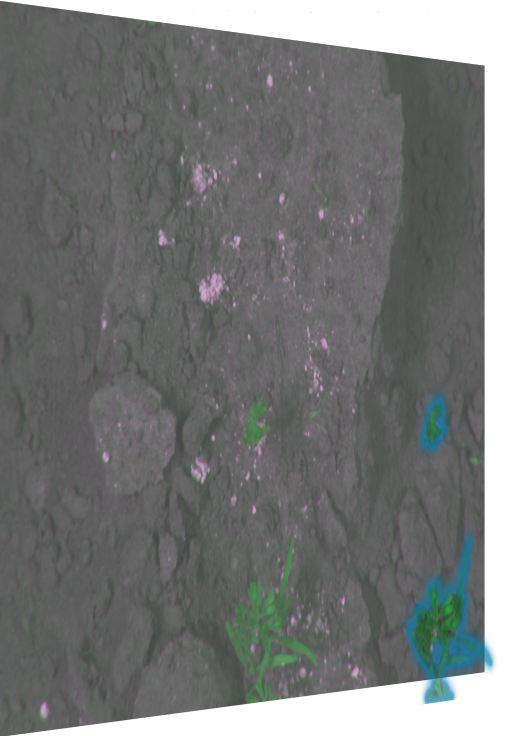
\includegraphics[width=0.5\textwidth]{imgs/fore_vs_back.png}
\caption{Foreground vs background.}
\label{fig:fore_vs_back}
\end{figure}

\subsection{Segment Anything}

The Segment Anything Model (SAM) utilises a transformer-based architecture~\cite{attention-Nips17}, which has been shown to be highly effective in natural language processing~\cite{GPT-3} and image recognition tasks~\cite{ViT2020}. Specifically, SAM uses a vision transformer-based \textbf{image encoder} to extract image features and \textbf{prompt encoders} to incorporate user interactions, followed by a \textbf{mask decoder} to generate segmentation results and confidence scores based on the image embedding, prompt embedding, and output token. 

\begin{figure}[h!]
\centering
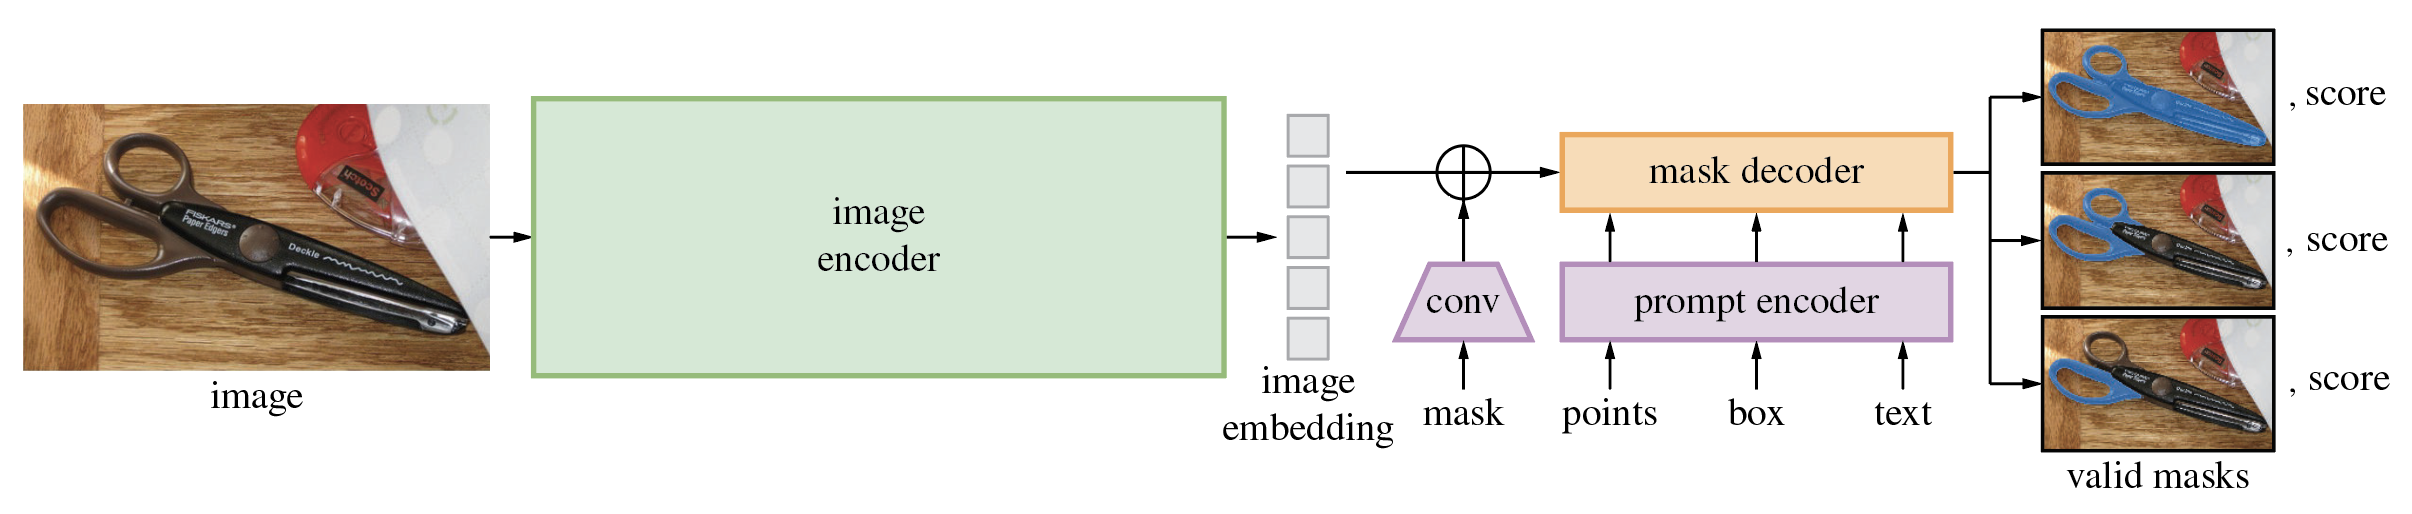
\includegraphics[scale=0.5,width=0.95\textwidth]{imgs/SAM_model_diagram.png}
\caption{Segment Anything Model (SAM) overview. A heavyweight image encoder outputs an image embedding that can
then be efficiently queried by a variety of input prompts to produce object masks.}
\label{fig:sam-diagram}
\end{figure}

The prompt encoders are tailored for different user inputs. SAM supports four different prompts: points, boxes, texts, and masks. Each point is encoded by Fourier positional encoding~\cite{FourierPE-Nips20} and two learnable tokens for specifying foreground and background, respectively. The bounding box is encoded by the point encoding of its top-left corner and bottom-right corner. The free-form text is encoded by the pre-trained text-encoder in CLIP~\cite{CLIP-ICML2021}. The mask prompt has the same spatial resolution as the input image, which is encoded by convolution feature maps. 
Finally, the mask decoder employs a lightweight design, which consists of two transformer layers with a dynamic mask prediction head and an Intersection-over-Union (IoU) score regression head. The mask prediction head can generate three 4$\times$ downscaled masks, which correspond to the whole object, part, and subpart of the object, respectively.

\begin{figure}[h!]
\centering
\begin{subfigure}[b]{.45\linewidth}
    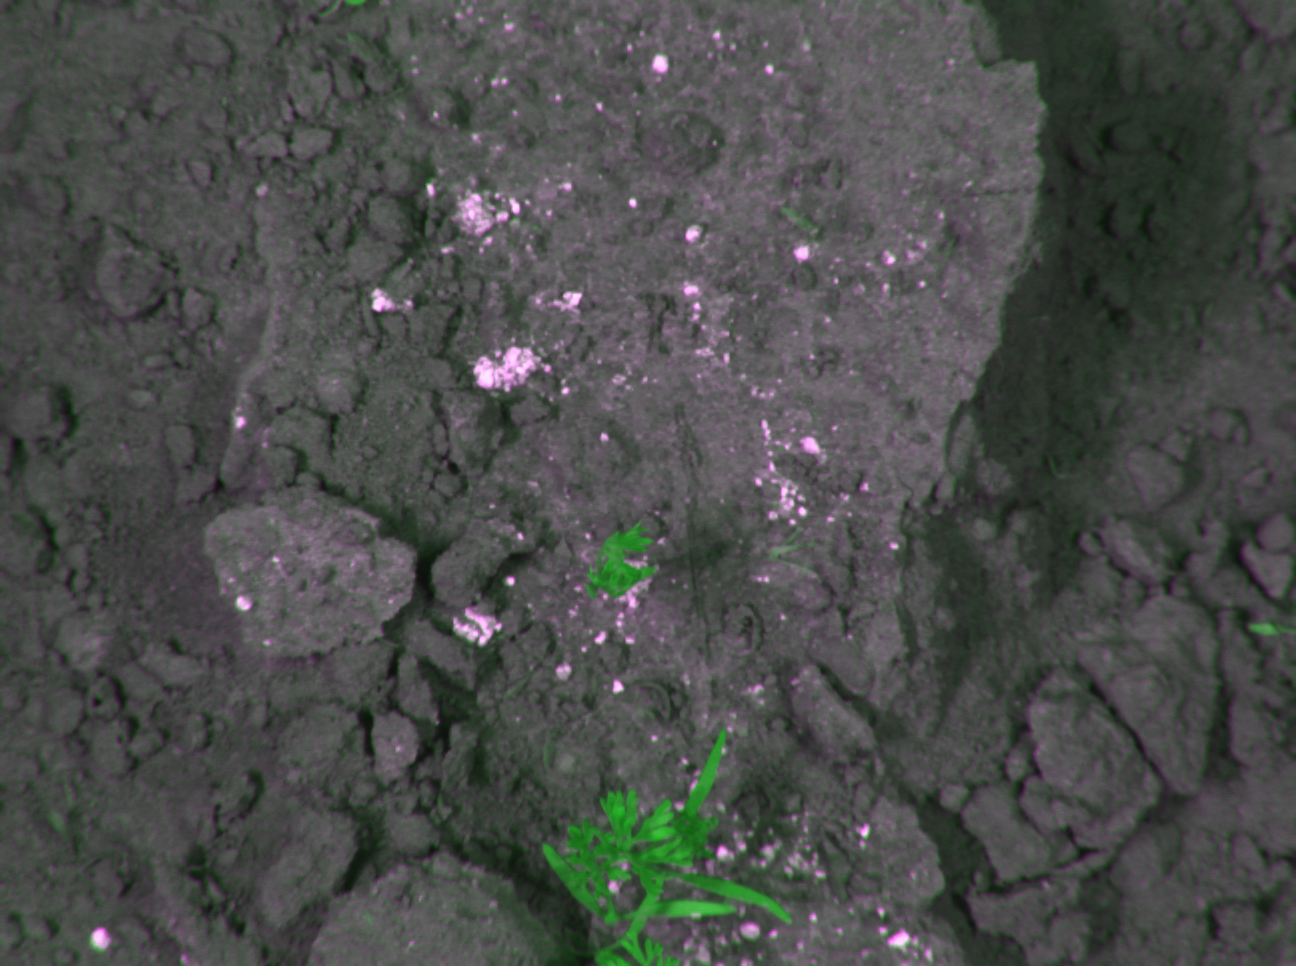
\includegraphics[width=\linewidth]{imgs/segmentation_modes_original.png}
    \caption{Original image}
\end{subfigure}
\begin{subfigure}[b]{.45\linewidth}
    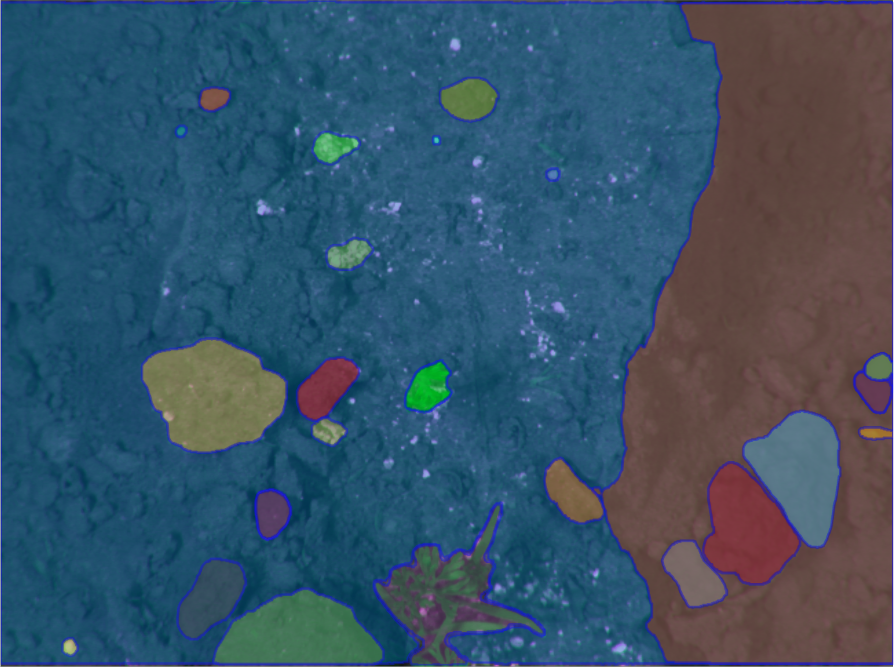
\includegraphics[width=\linewidth]{imgs/segmentation_modes_everything.png}
    \caption{Fully automatic mode}
\end{subfigure}

\begin{subfigure}[b]{.45\linewidth}
    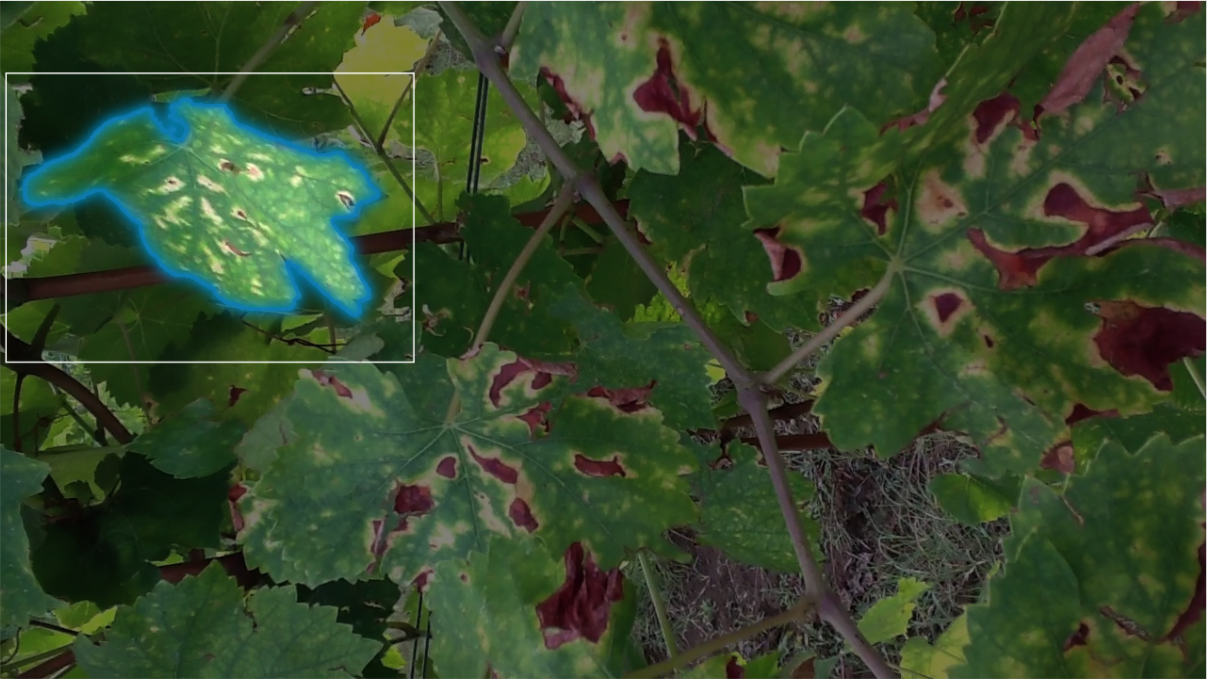
\includegraphics[width=\linewidth]{imgs/segmentation_modes_bbox.png}
        \caption{Bounding box mode}
\end{subfigure}
\begin{subfigure}[b]{.45\linewidth}
   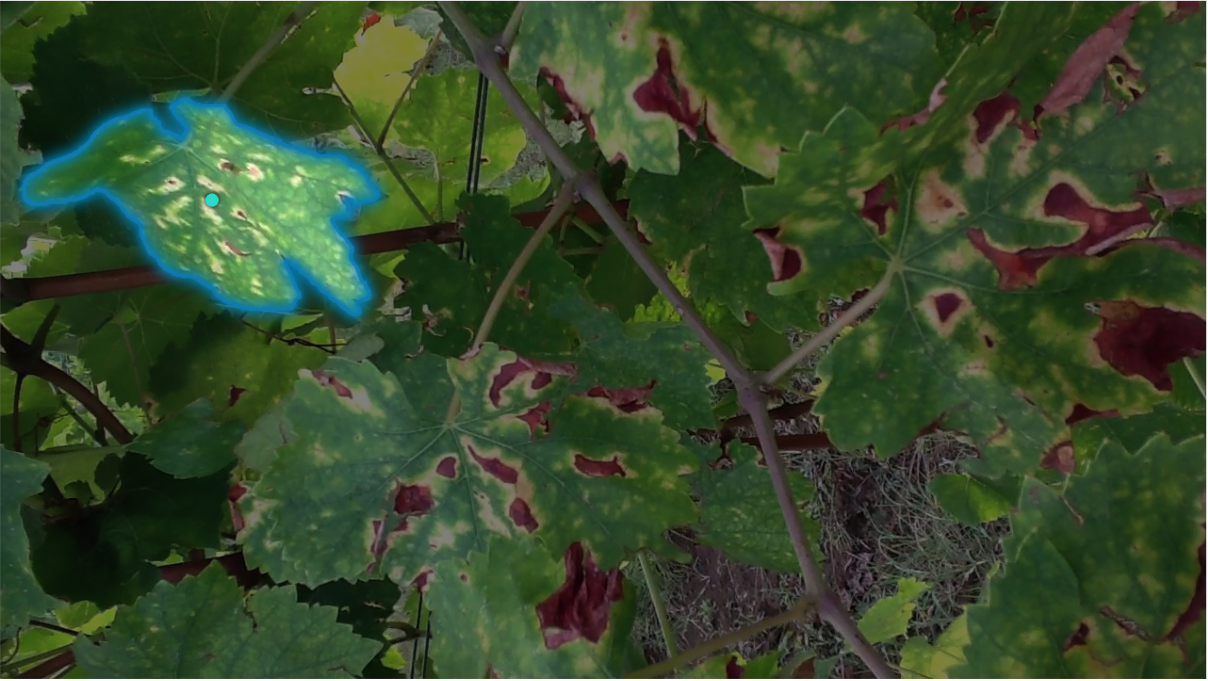
\includegraphics[width=\linewidth]{imgs/segmentation_modes_1point.png}
   \caption{Additional point modality}
\end{subfigure}
%\begin{subfigure}[b]{.33\linewidth}
%    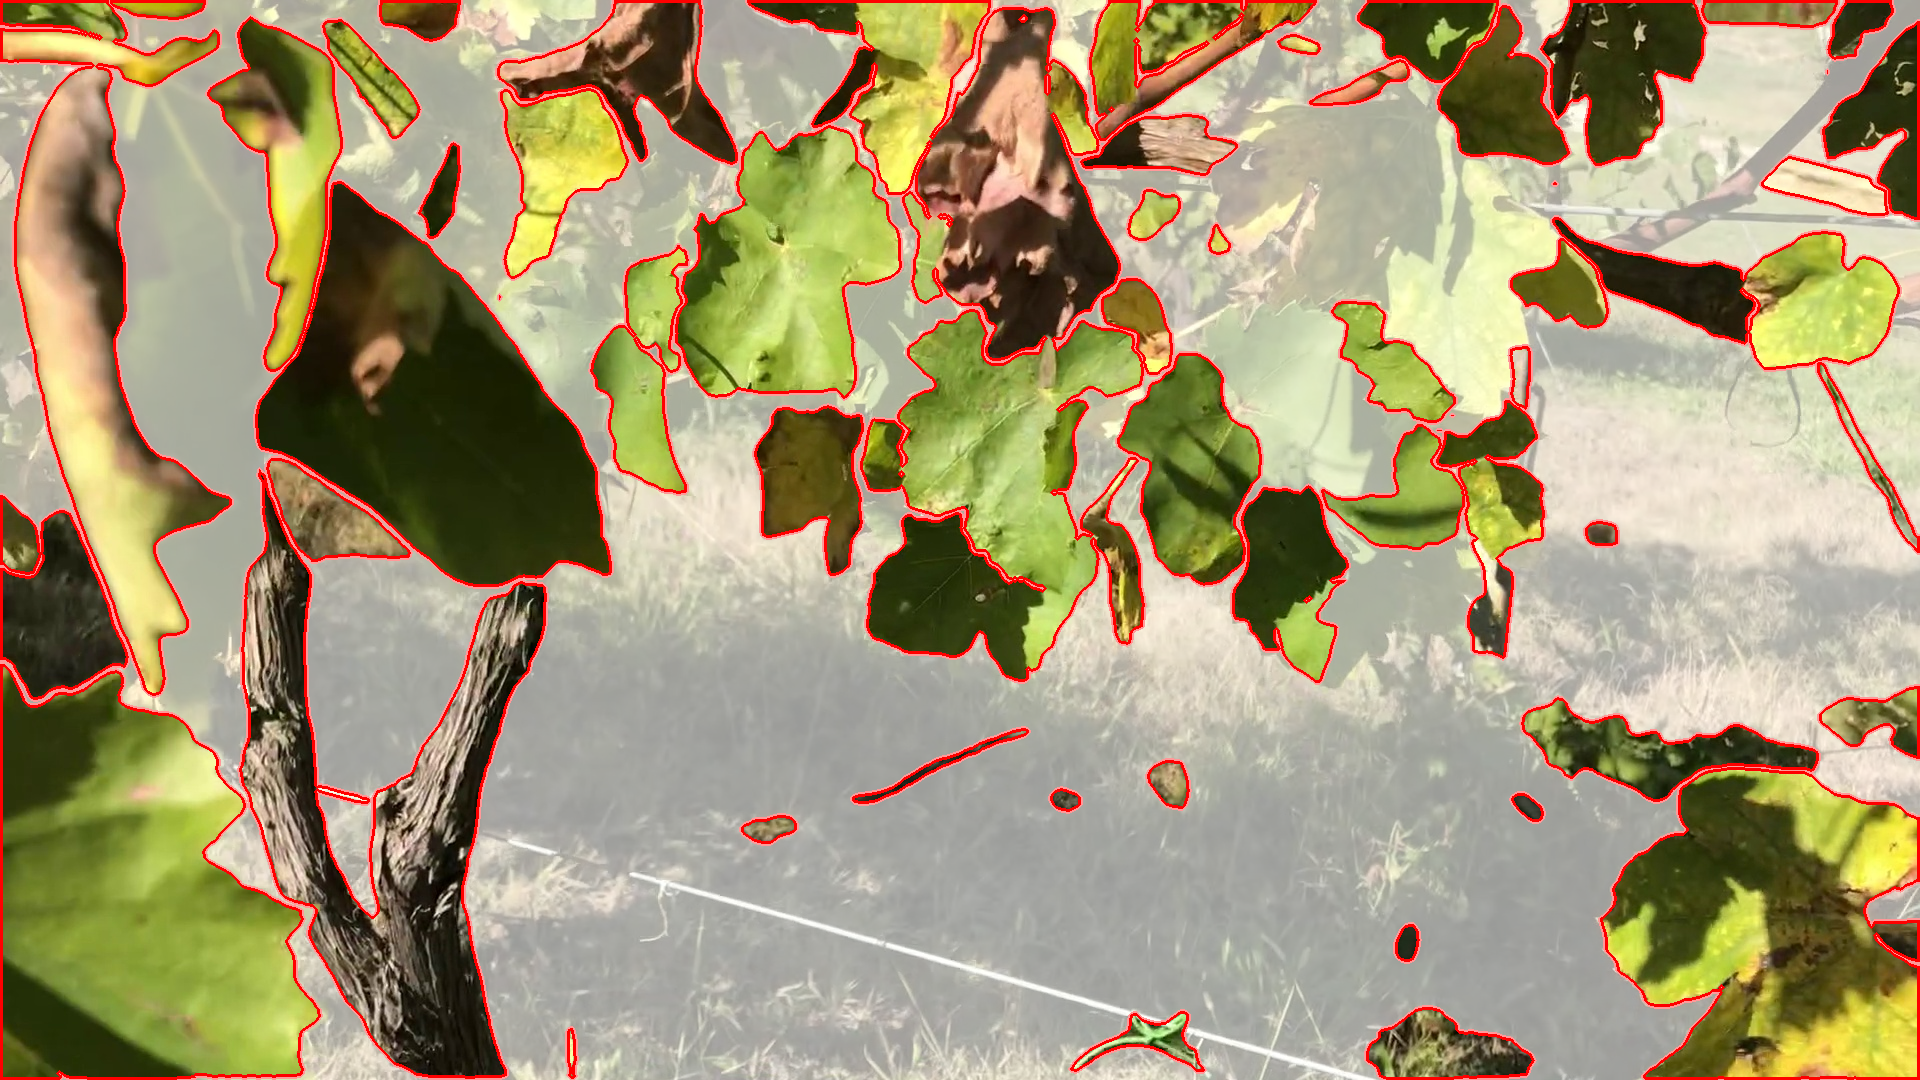
\includegraphics[width=\linewidth]{imgs/healthy_033_cam3_mask_over_healthy_033_cam3.png}
%\end{subfigure}
\caption{Segmentation results of SAM based on different segmentation modes.}
\label{fig:sam-modes}
\end{figure}

To summarize, when applying SAM for agricultural image segmentation, the segment-everything mode is prone to generate useless region partitions and the point-based mode is ambiguous and requires multiple prediction-correction iterations. In contrast, the bounding box-based mode can clearly specify the ROI and obtain reasonable segmentation results without multiple trials and errors. We argue that the bounding box-based segmentation mode has wider practical values than the segment-everything and point-based mode when using SAM in medical image segmentation tasks.

Since the image encoder can be applied prior to prompting the model, we can pre-compute the image embedding for all training images to avoid replicated computing of the image embedding per prompt, which can significantly improve the training efficiency. The mask decoder only needs to generate one mask rather than three masks because the bounding box prompt can clearly specify the expected segmentation target in most situations. 

\subsection{U-Net and EfficientNet}

U-Net is a Convolutional Neural Network (CNN) originally proposed for the segmentation of biomedical images~\cite{ronneberger2015unet}.  Afterwards the same net has been used for tackling segmentation of Urban Environment surfaces from High Resolution Satellite Imagery~\cite{McGlinchy2019}. Variations of U-Net have been used in precisoin agriculture, for example to segment cucumber leaves with disease spots \cite{WANG2021106373}, or images of Cichorium intybus L. root~\cite{smith_segmentation_2020}.

%perform environmental microorganism image segmentation \cite{ZHANG2021107885}. Further modifications have been used to segment cucumber leaves with disease spots \cite{WANG2021106373} and to tackle Iris segmentation \cite{LIAN2018296} with occurrence of occlusion and reflection problems, blurring and poor or overexposed illumination. The use of U-Net covers also segmentation of Cichorium intybus L. root images \cite{smith_segmentation_2020}.

The U-Net architecture is, specifically, a Fully Convolutional Neural Network (FCNN) model commonly used for semantics segmentation and instance segmentation tasks. This architecture derives its name from its U-shaped structure (Figure~\ref{fig:unet}) consisting of two main parts, from left to right: the contracting path (encoder) and the expanding path (decoder). The contracting path of U-Net consists of multiple convolutional and pooling layers. These layers gradually reduce the spatial dimensions while increasing the number of feature channels, which helps capture a wide range of features at different scales. Each contracting block typically consists of two convolutional layers followed by a downsampling operation such as max pooling. The expanding path is the decoder part of U-Net and is responsible for generating the segmentation map. It consists of upconvolutional (also known as transposed convolutional) layers, which perform upsampling and increase the spatial dimensions. The expanding path also includes skip connections that concatenate feature maps from the corresponding contracting path. These skip connections enable the decoder to access the high-resolution feature maps from the encoder, aiding in the precise localization of objects. At the end of the U-Net architecture, a final convolutional layer is typically applied to produce the segmentation map with the desired number of output channels, representing the class probabilities or pixel-wise labels. 

\begin{figure}[h!]
\centering
   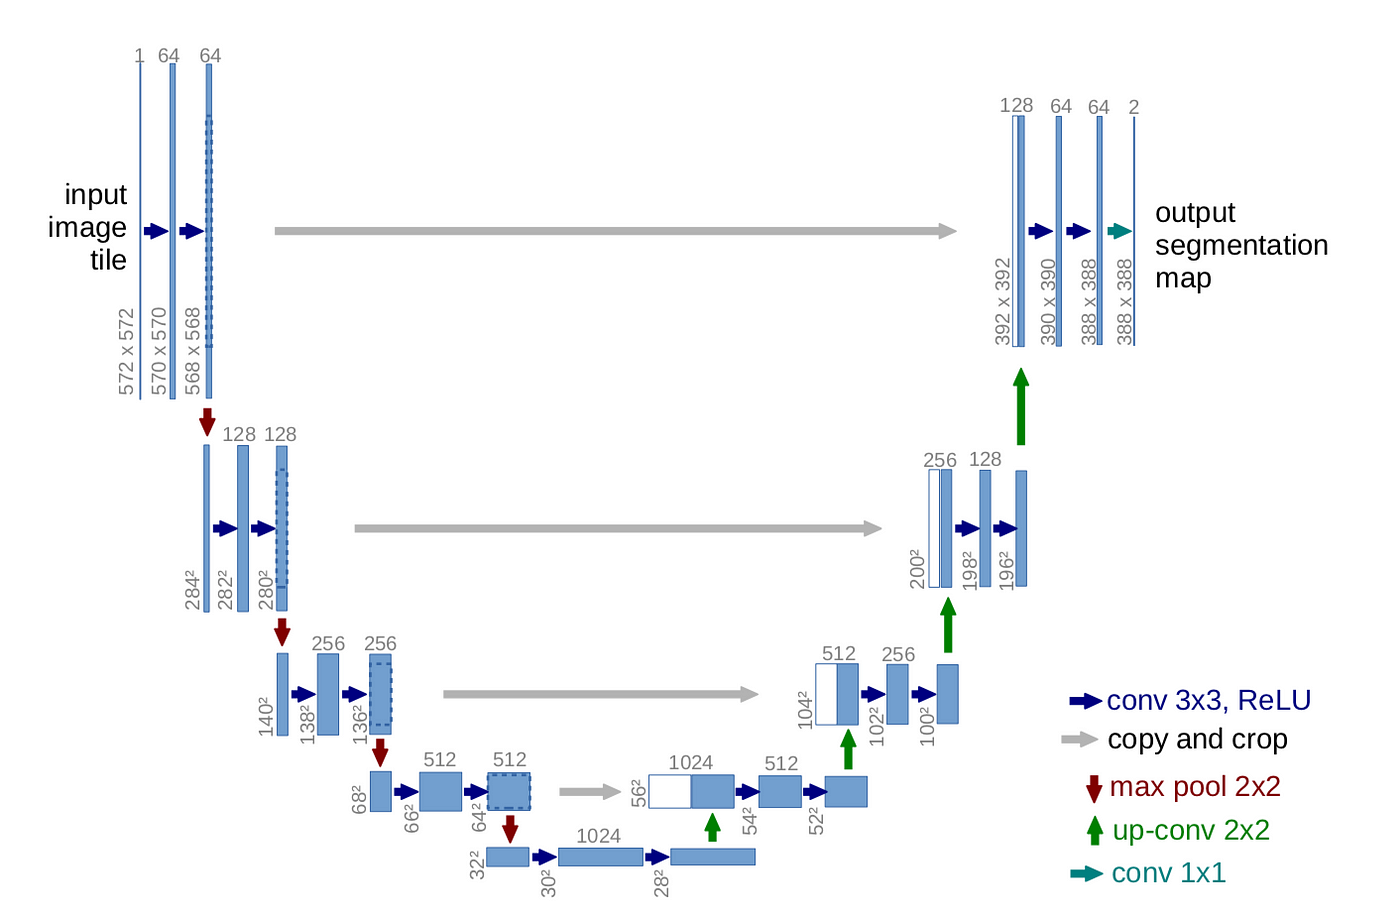
\includegraphics[width=\linewidth]{imgs/U_Net.png}
\caption{U-net architecture% (example for 32$\times$32 pixels in the lowest resolution). Each blue
%box corresponds to a multi-channel feature map. The number of channels is denoted
%on top of the box. The x-y-size is provided at the lower left edge of the box. White
%boxes represent copied feature maps. The arrows denote the different operations.
}
\label{fig:unet}
\end{figure}

EfficientNet~\cite{EfficientNet} is a family of convolutional neural network (CNN) models that are designed to achieve state-of-the-art performance while being highly efficient in terms of computational resources.

EfficientNet models are based on a concept called compound scaling, which optimizes the depth, width, and resolution of the network to achieve a good balance between accuracy and efficiency.  The compound scaling technique involves uniformly scaling the network width, depth, and resolution using a coefficient called the compound scaling factor. This factor ensures that all dimensions of the network grow proportionally. By scaling up the network, it captures more complex patterns and features, while scaling down reduces the number of parameters and computations required. EfficientNet models have achieved state-of-the-art performance on various computer vision tasks, including image classification, object detection, and segmentation, across different benchmark datasets. They have demonstrated superior accuracy compared to other popular CNN architectures, such as ResNet, while maintaining high efficiency in terms of memory usage and computational requirements.

%\cite{Learning_for_Structured_Prediction}

EfficientNet models are often used as a backbone or encoder in various architectures, such as UNet, to improve performance and efficiency in tasks like image segmentation. The UNet architecture with an EfficientNet encoder combines the strengths of both models to achieve highly efficient and accurate image segmentation: it has been used in biomedical applications~\cite{le2022cell}~\cite{liu_automatic_2022} and it is implemented in the  APEER ML toolkit by {\color{red}{Zeiss\textsuperscript{\tiny\textregistered}}}(\cite{Zeiss23}).

The UNet architecture, known for its U-shaped design, and EfficientNet, a state-of-the-art convolutional neural network (CNN) model, complement each other to improve performance. The EfficientNet encoder serves as the backbone of the network and is responsible for capturing high-level features from the input image. EfficientNet models are known for their superior performance and efficiency by leveraging compound scaling, which optimizes the depth, width, and resolution of the network based on a given resource constraint. In the UNet architecture, the contracting path (encoder) is responsible for capturing context and extracting features at different scales, while the expanding path (decoder) performs precise localization using skip connections. In the UNet with EfficientNet encoder, the contracting path is replaced with the EfficientNet backbone. The EfficientNet encoder provides a powerful feature extraction capability, capturing both low-level and high-level features from the input image. The extracted features are then passed to the expanding path, where upsampling and skip connections are used to recover the spatial resolution and refine the segmentation output.

%By combining the UNet architecture with the EfficientNet encoder, the model benefits from the efficient and accurate feature extraction capabilities of EfficientNet, along with the precise localization ability of UNet. This combination enables the network to effectively handle complex image segmentation tasks while maintaining efficiency in terms of memory usage and computational resources.
%
%Overall, the UNet with EfficientNet encoder architecture offers a powerful and efficient solution for image segmentation tasks, leveraging the strengths of both models to achieve superior performance.

\begin{figure}[h!]
\centering
   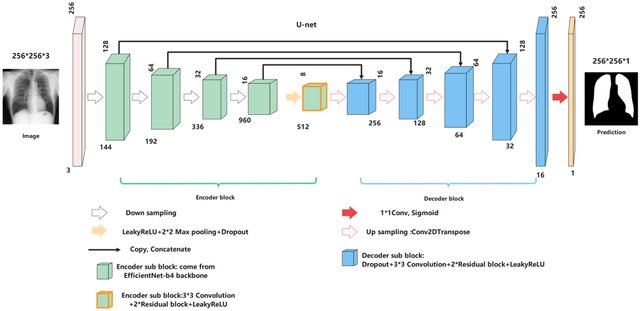
\includegraphics[width=\linewidth]{imgs/U-Net-with-EfficientNet-b4-Encoder_W640.jpg}
\caption{U-Net architecture with EfficientNet encoder~\cite{liu_automatic_2022}}
\label{fig:efficientnet}
\end{figure}

\section{Experiments and Results}

The ESCA dataset~\cite{ESCA_dataset} contains 1770 RGB images in jpg format taken at a working distance of approximately 30 cm from grapevine plants during sunny and windy days and considering scenarios with background variety. In 882 of these images, the totality of plants appearing therein is healthy (not affected by Esca). In contrast, the other 888 images contain at least one depiction of shoots with visible foliar symptoms of Esca disease. The ESCA dataset consists of two folders, esca and healthy, each containing images of the relative class.

Deep neural networks require large amounts of training data to tune millions of parameters and develop a learned model for subsequent predictions. While it is possible to crowdsource image annotation for natural scenes and collect large datsets as shown in Table~\ref{tab:models_datasets}, it is difficult to find experts to annotate images for specific scientific domains. Each research topic requires researchers to annotate their own images. Annotation being a very time consuming task, a researcher can end up with a handful of annotated images containing only tens of labeled objects. 

Our goal was to compare the performances of the foundational segmentation model SAM with no training to the previously available segmentation model U-Net, which requires manual annotation. The chosen task is semantic segmentation i.e. to classify the pixels of each image into two different semantic categories: foliage and background. This task could be an important first part in a Machine Learing pipeline whose later stages focus on the analysis of the Region of Interest inside the pictures, which in this case we considered to be the area occupied by foliage.

\begin{figure}[h!]
\centering
\begin{subfigure}[b]{.47\linewidth}

\includegraphics[width=\linewidth]{imgs/placeholder.jpg}
\caption{}
\label{fig:sam1a}
\end{subfigure}
\begin{subfigure}[b]{.47\linewidth}

\includegraphics[width=\linewidth]{imgs/placeholder.jpg}
\caption{}
\label{fig:sam1b}
\end{subfigure}
\caption{Ground truth segmentation of foliage (hand-made mask) for {\color{red}healthy1.jpg} and {\color{red}esca1.jpg}}
\label{fig:true_segmentation}
\end{figure}

We uploaded {\color{red} 102} images of the healthy folder and {\color{red} 103} of the esca folder to \url{https://www.apeer.com/annotate} and  manually annotated them with the online semantic segmentation tool APEER Annotate~\cite{Zeiss23}, which allowed to classify the pixels of each image into two different semantic categories: foliage and background. The reult of the manual sementation are a total of {\color{red} 205} binary masks in which the pixels corresponding to foliage area contain the value 1 and all others contain value 0.



\begin{table}[h!]
\centering
\begin{tabular}{|p{3.0cm}|p{3.5cm}|}
\hline
\makecell{\textbf{Image name}} 
& 
\makecell{\textbf{Manual annotation time} \\ \textbf{(minutes)}} \\
\hline
healthy1.jpg & xx \\
\hline
healthy2.jpg & xx \\
\hline
healthy3.jpg & xx \\
\hline
healthy4.jpg & xx \\
\hline
healthy5.jpg & xx \\
\hline
esca1.jpg & xx \\
\hline
esca2.jpg & xx \\
\hline
esca3.jpg & xx \\
\hline
esca4.jpg & xx \\
\hline
esca5.jpg & xx \\
\hline
\end{tabular}
\caption{Time spent for drawing the masks manually (ground-truth labelling).}
\label{tab:image_annotation_on_apeer}
\end{table}

In Table~\ref{tab:image_annotation_on_apeer} we recorded the time used to manually draw precise segmentation masks for 10 images. We keep the so-obtained 10 masks as a reference for the rest of the paper and consider them as ground-truth to measure performance of the two segmentation tools analyzed. In~\ref{tab:definitions} we summarized the classification of pixel predictions in the context of semantic segmentation applied to the task of partitioning an image into its Region Of Interest (ROI) and its background.{\color{red} Frase contorta.}

\begin{table}[h!]
\centering
\begin{tabular}{|p{4.5cm}|p{4.5cm}|}
\hline
\makecell{\textbf{Correct predictions}}
&
\makecell{\textbf{Incorrect predictions}} \\
\hline

True Positive (TP):
the pixel has been predicted as part of the ROI and
actually belongs to the ROI 

 & 

False Positive (FP):
the pixel has been predicted as part of the ROI but 
does not belong to the ROI \\

\hline

True Positive (TN):
the pixel has been predicted as part of the background and
actually belongs to the background  

& 

True Positive (FN):
the pixel has been predicted as part of the background but
actually belongs to the ROI  \\

\hline
\end{tabular}
\caption{Definitions of TP, TN, FP, and FN}
\label{tab:definitions}
\end{table}

The metrics used in this paper are:
\begin{itemize}
\item Intersection over Union (IoU) or Jaccard Index: it measures the overlap between the predicted segmentation mask and the ground truth mask. It is calculated as the ratio of the intersection area to the union area of the two masks (in the case of two classes only this measure is equivalent to Mean Intersection over Union - mIoU).
\item Dice Coefficient (DC): It measures the similarity between the predicted boundaries and the ground truth boundaries. It calculates the ratio of twice the intersection of the boundaries to the sum of their areas.
\item Pixel Accuracy (PA): it measures the percentage of correctly classified pixels compared to the total number of pixels in the image. It calculates the overall accuracy of the segmentation.
\item Precision, Recall, and F1-score: these metrics are commonly used in multi-class semantic segmentation evaluation. Precision measures the proportion of correctly classified positive pixels, recall measures the proportion of actual positive pixels that are correctly classified, and F1-score combines precision and recall to provide a balanced measure.
\item Normalized Surface Distance (NSD): the average of the Hausdorff distance and the Symmetric Contour Distance. Hausdorff Distance: The Hausdorff distance measures the maximum distance between the predicted contour and the ground truth contour. It quantifies the largest discrepancy between the two contours and is sensitive to outliers or large deviations. Symmetric Contour Distance: The symmetric contour distance measures the average distance between the predicted contour and the ground truth contour. Unlike the Hausdorff distance, it takes into account both the under-segmentation (missing parts of the object) and over-segmentation (extraneous regions).
\end{itemize}

\subsection{Segmentation of vine images with SAM}

SAM supports three main segmentation modes: segmenting everything in a fully automatic way, bounding box mode, and point mode. The segment-everything mode divides the whole image into six regions based on the image intensity (Fig.~\ref{fig:sam-modes}b).

We segmented {\color{red} 10} images with bounding box mode and other {\color{red} 10} images with point mode. These modes are semi-automatic, i.e. they require a human input for each image.

\begin{table}[h!]
\centering
\begin{tabular}{|p{3.0cm}|p{3.0cm}|p{3.0cm}|}
\hline
\makecell{\textbf{Image name}}  
&
\makecell{\textbf{Annotation time} \\ \textbf{bounding box mode}}
&
\makecell{\textbf{Annotation time} \\ \textbf{point mode}}\\
& 
\makecell{\textbf{(minutes)}}
& 
\makecell{\textbf{(minutes)}} \\
\hline
healthy1.jpg & xx & xx \\
\hline
healthy2.jpg & xx & xx \\
\hline
healthy3.jpg & xx & xx \\
\hline
healthy4.jpg & xx & xx \\
\hline
healthy5.jpg & xx & xx \\
\hline
esca1.jpg & xx & xx \\
\hline
esca2.jpg & xx & xx \\
\hline
esca3.jpg & xx & xx \\
\hline
esca4.jpg & xx & xx \\
\hline
esca5.jpg & xx & xx \\
\hline
\end{tabular}
\caption{Time spent to identify object masks with SAM using its semi-automatic modes.}
\label{tab:image_annotation_on_SAM_manual}
\end{table}

Figure~\ref{fig:sam-modes} shows the results of the three segmentation modes on an image of vines from the ESCA dataset~\cite{ESCA_dataset} and Table~\ref{tab:image_annotation_on_SAM_manual} reports the exact time necessary to manually draw segmentation masks for the 10 selected images~\footnote{The results are based on the online demo: \url{https://segment-anything.com/demo}.}.

We launched a batch segmentation job exploiting the fully-automatic mode on the entire set of 1770 images of the Esca dataset, using as hardware platform an NVIDIA RTX\textsuperscript{\texttrademark} A6000 GPU. For the instantiation of the model we adopted the {\tt ViT-H}~\cite{ViT-H} checkpoint. SAM produced for each segmented image a folder containing one mask for each object found in the image (between 100 and 200 objects). In order to process 888 images of the esca folder took 55 minutes and 13.8 seconds. In order to process 882 images of the healthy folder took 69 minutes and 19.4 seconds to complete the merge of masks took 48 minutes and 45.4 seconds to complete.

%%%%%%%%%%
% It does not make sense to record segmentation time of individual images.
% We just report global time  of segmentation for the entire dataset
%%%%%%%%%%
\begin{table}[h!]
\centering
\begin{tabular}{|p{3.0cm}|p{3.0cm}|p{3.5cm}|p{3.5cm}|}
\hline
 &  & \multicolumn{2}{c|}{\textbf{Image segmentation time (minutes)}} \\
\hline
\makecell{\textbf{Image folder}}
&
\makecell{\textbf{Number of images}}
&
\makecell{\textbf{Object segmentation} \\  \textbf{(automatic mode)}}
&
\makecell{\textbf{Object masks merging}} \\
\hline
Esca     & 888 & 55' and 13.8''   & ???  \\
\hline
Healthy & 882 &  69'' and 19.4'' & 48' and 45.4'' \\
\hline
\end{tabular}
\caption{Image segmentation time with SAM in automatic batch mode.}
\label{tab:image_segmentation_on_SAM_automatic}
\end{table}

%caThe project implies the public release three \emph{checkpoints} {\tt ViT-L} \cite{ViT-L}, {\tt ViT-B} \cite{ViT-B} and {\tt ViT-H} \cite{ViT-H}. Each checkpoint is a large file containing the weights for a deep neural network structure which has been obtained by training with different hyperparameters on the SA-1B dataset \cite{SA-1B_dataset}. The latter is the largest segmentation dataset to date, with over 1 billion masks on 11M licensed and privacy-respecting images. With the Segment Anything Model (SAM), the literature usually refers indistinctly to one of the three versions of the deep neural network created using one of the checkpoints. 

\begin{figure}[h!]
\centering
\begin{subfigure}[b]{.33\linewidth}
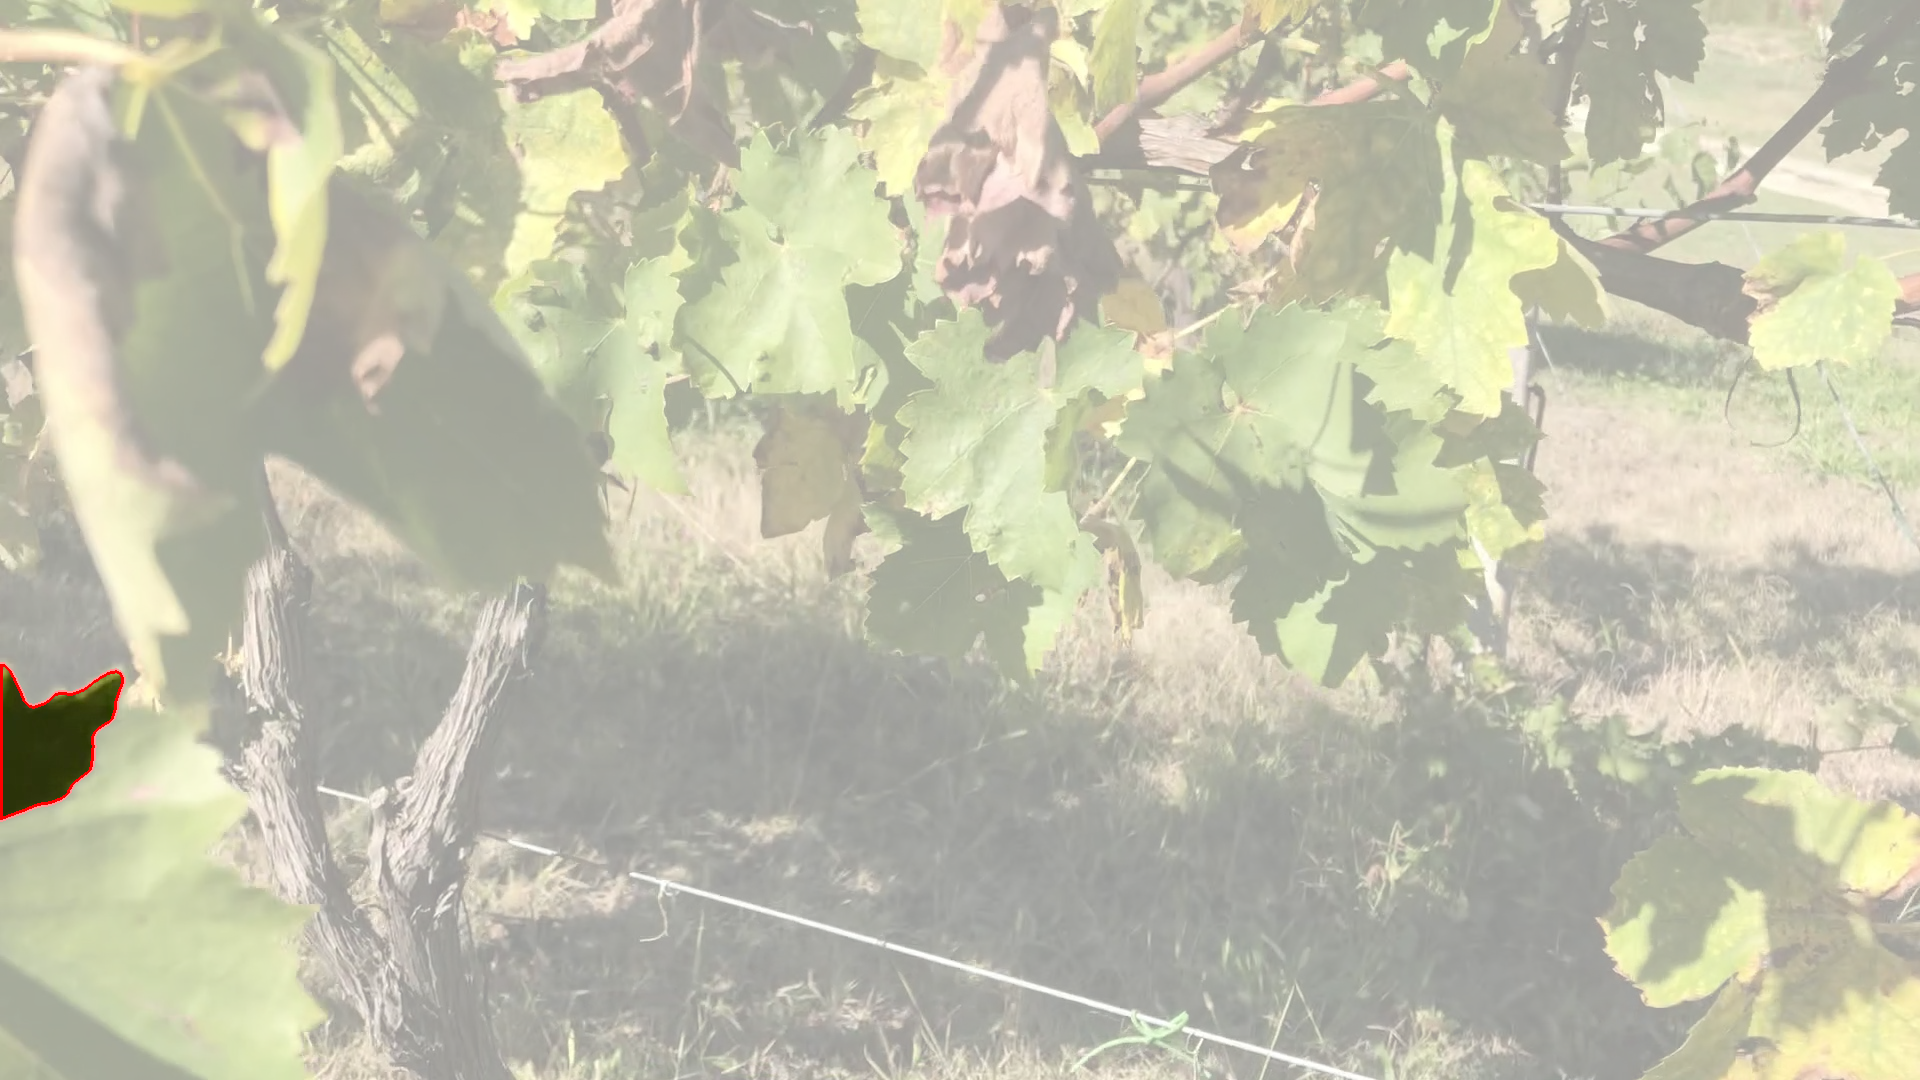
\includegraphics[width=\linewidth]{imgs/18_over_healthy_033_cam3.png}
\caption{}
\label{fig:sam1a}
\end{subfigure}
\begin{subfigure}[b]{.33\linewidth}
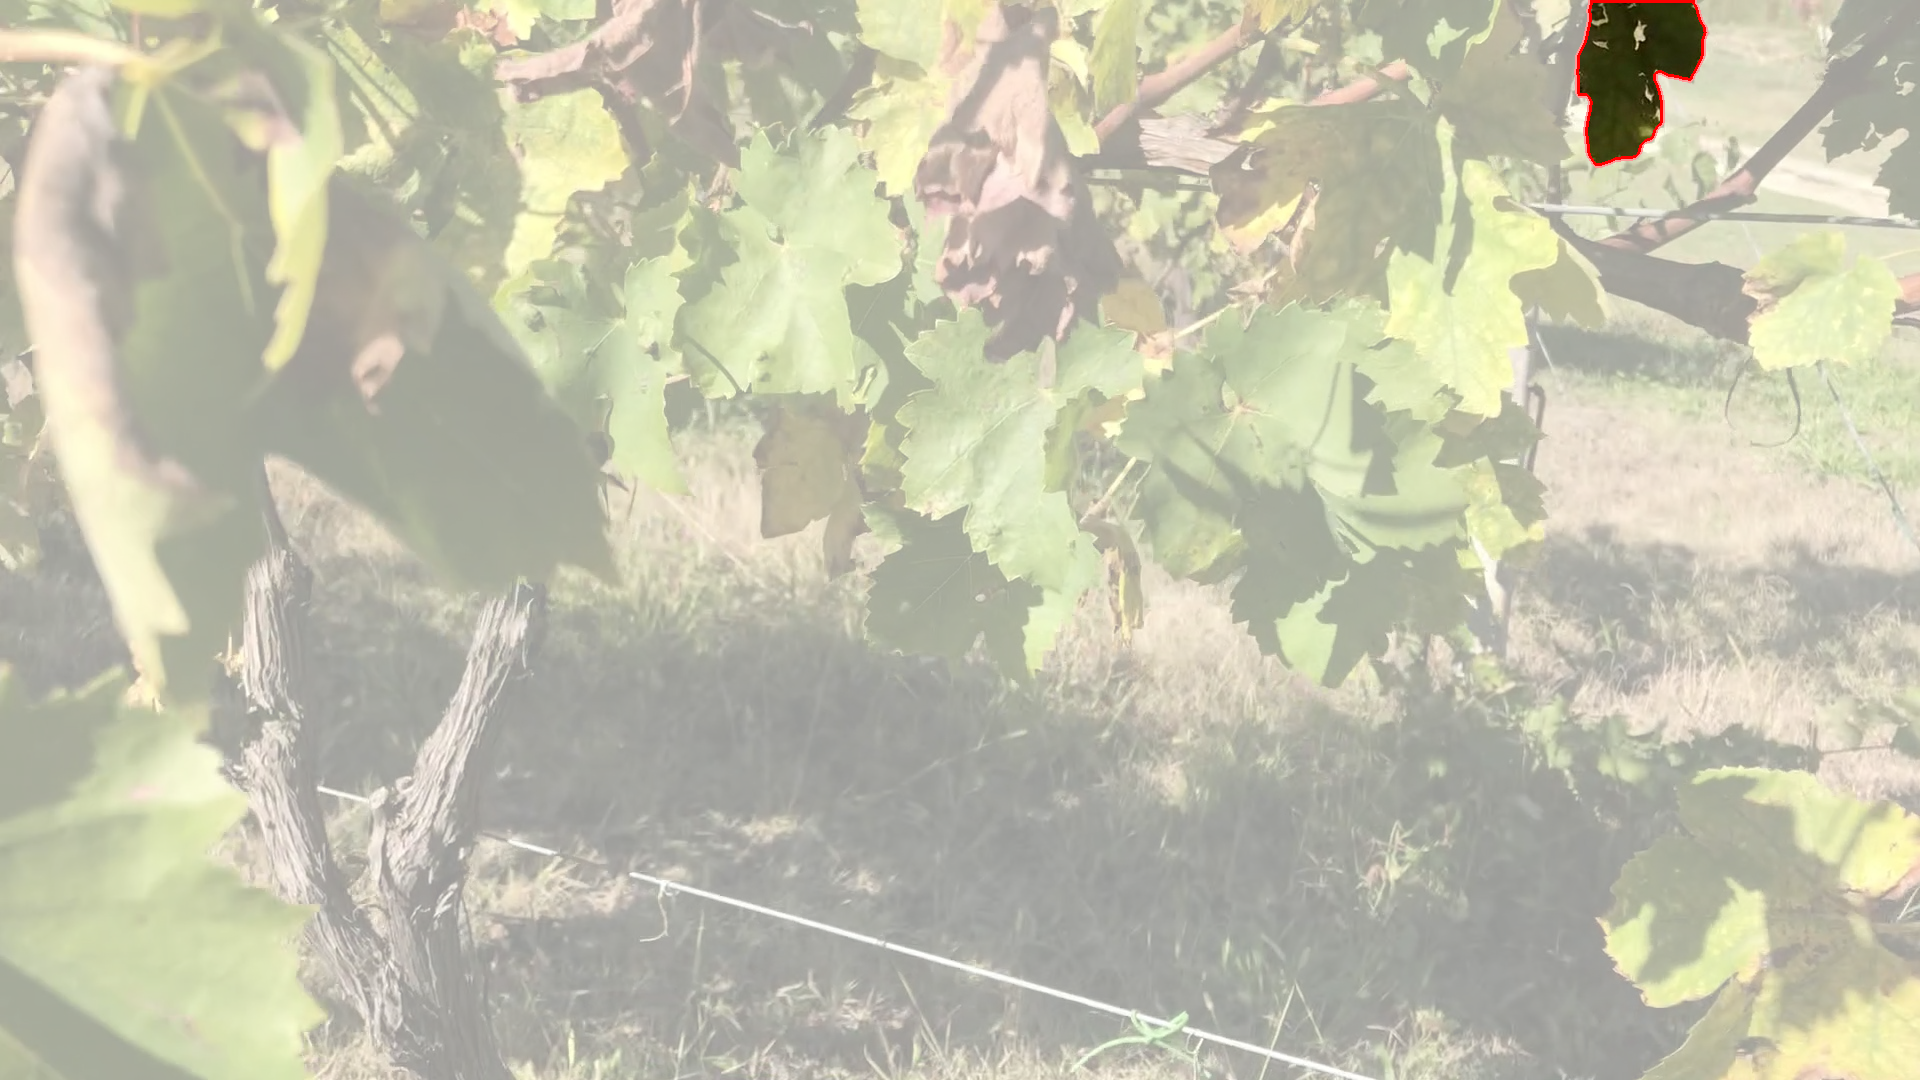
\includegraphics[width=\linewidth]{imgs/19_over_healthy_033_cam3.png}
\caption{}
\label{fig:sam1b}
\end{subfigure}%%%%%%%%%%%%%%%%%%%%%%%%%%%%%

%\begin{subfigure}[b]{.33\linewidth}
%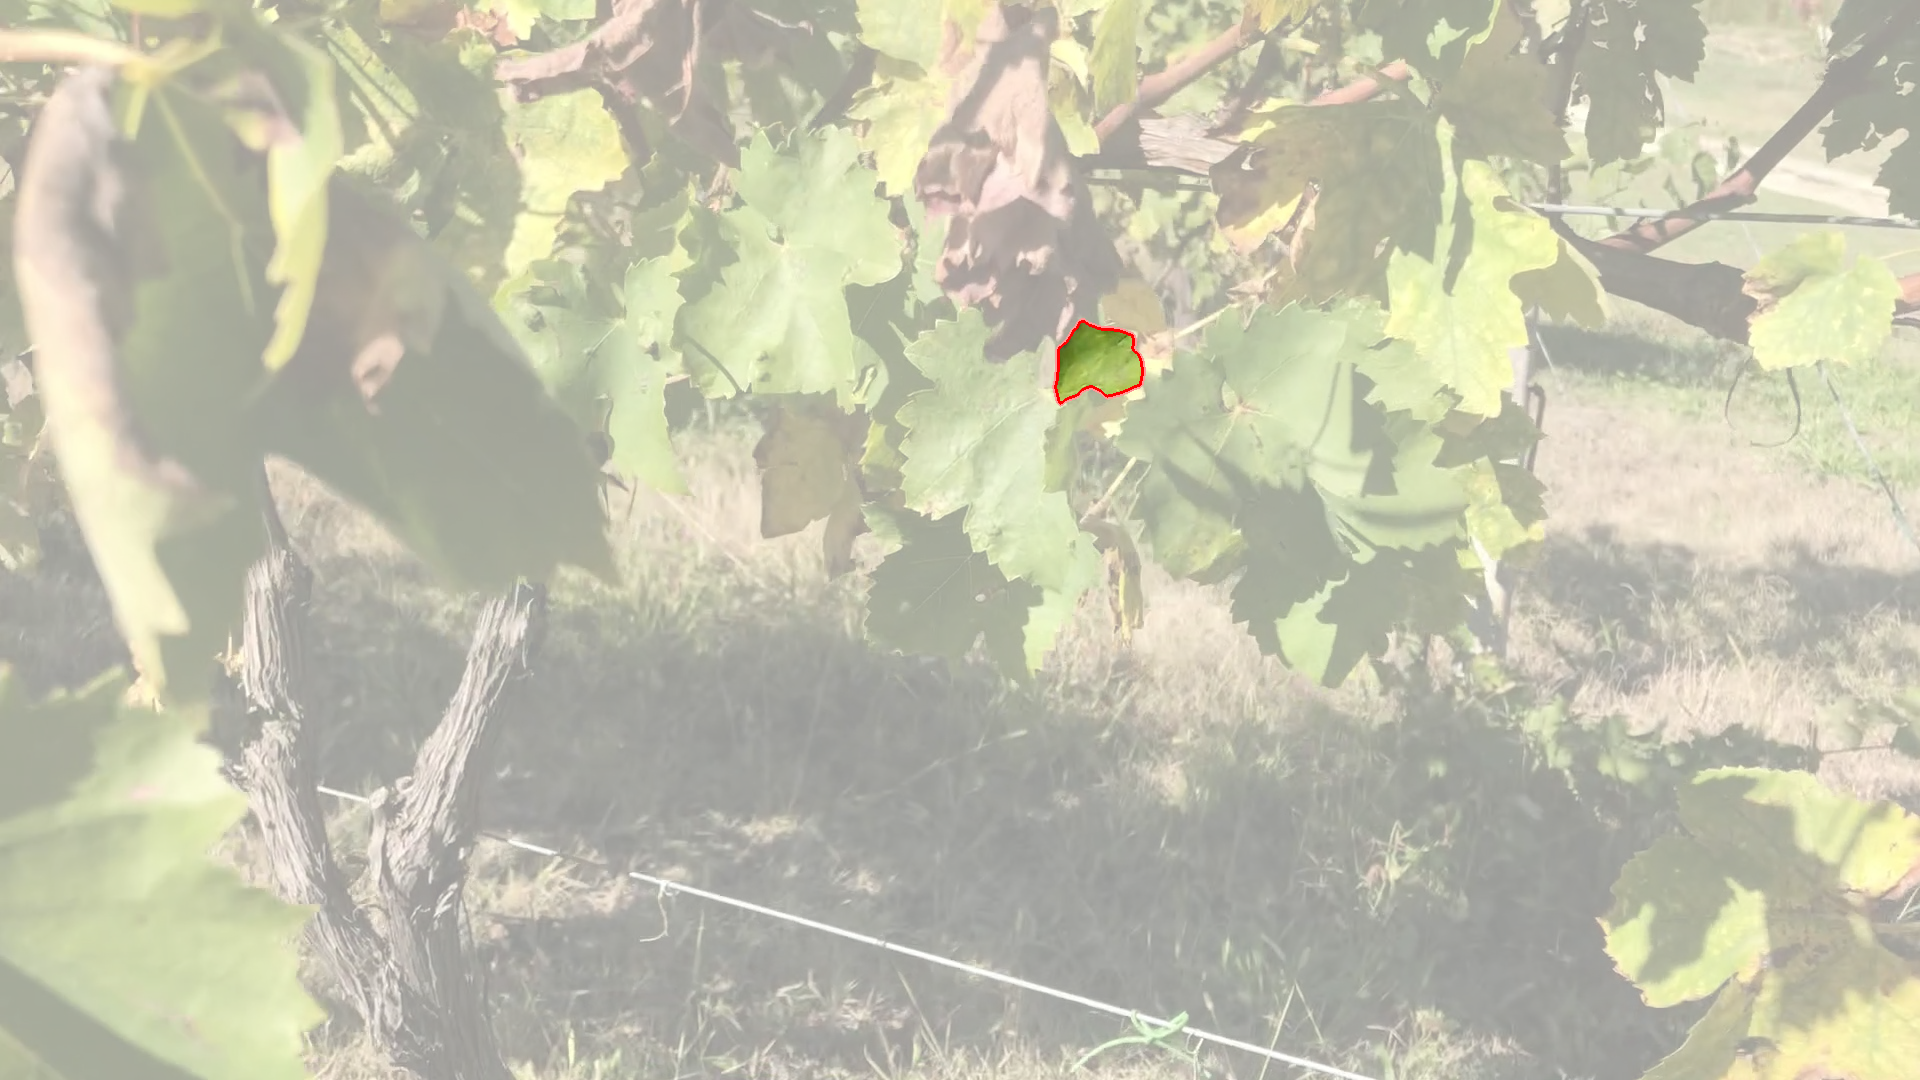
\includegraphics[width=\linewidth]{imgs/23_over_healthy_033_cam3.png}
%\caption{}
%\label{fig:sam1c}
%\end{subfigure}
%\begin{subfigure}[b]{.33\linewidth}
%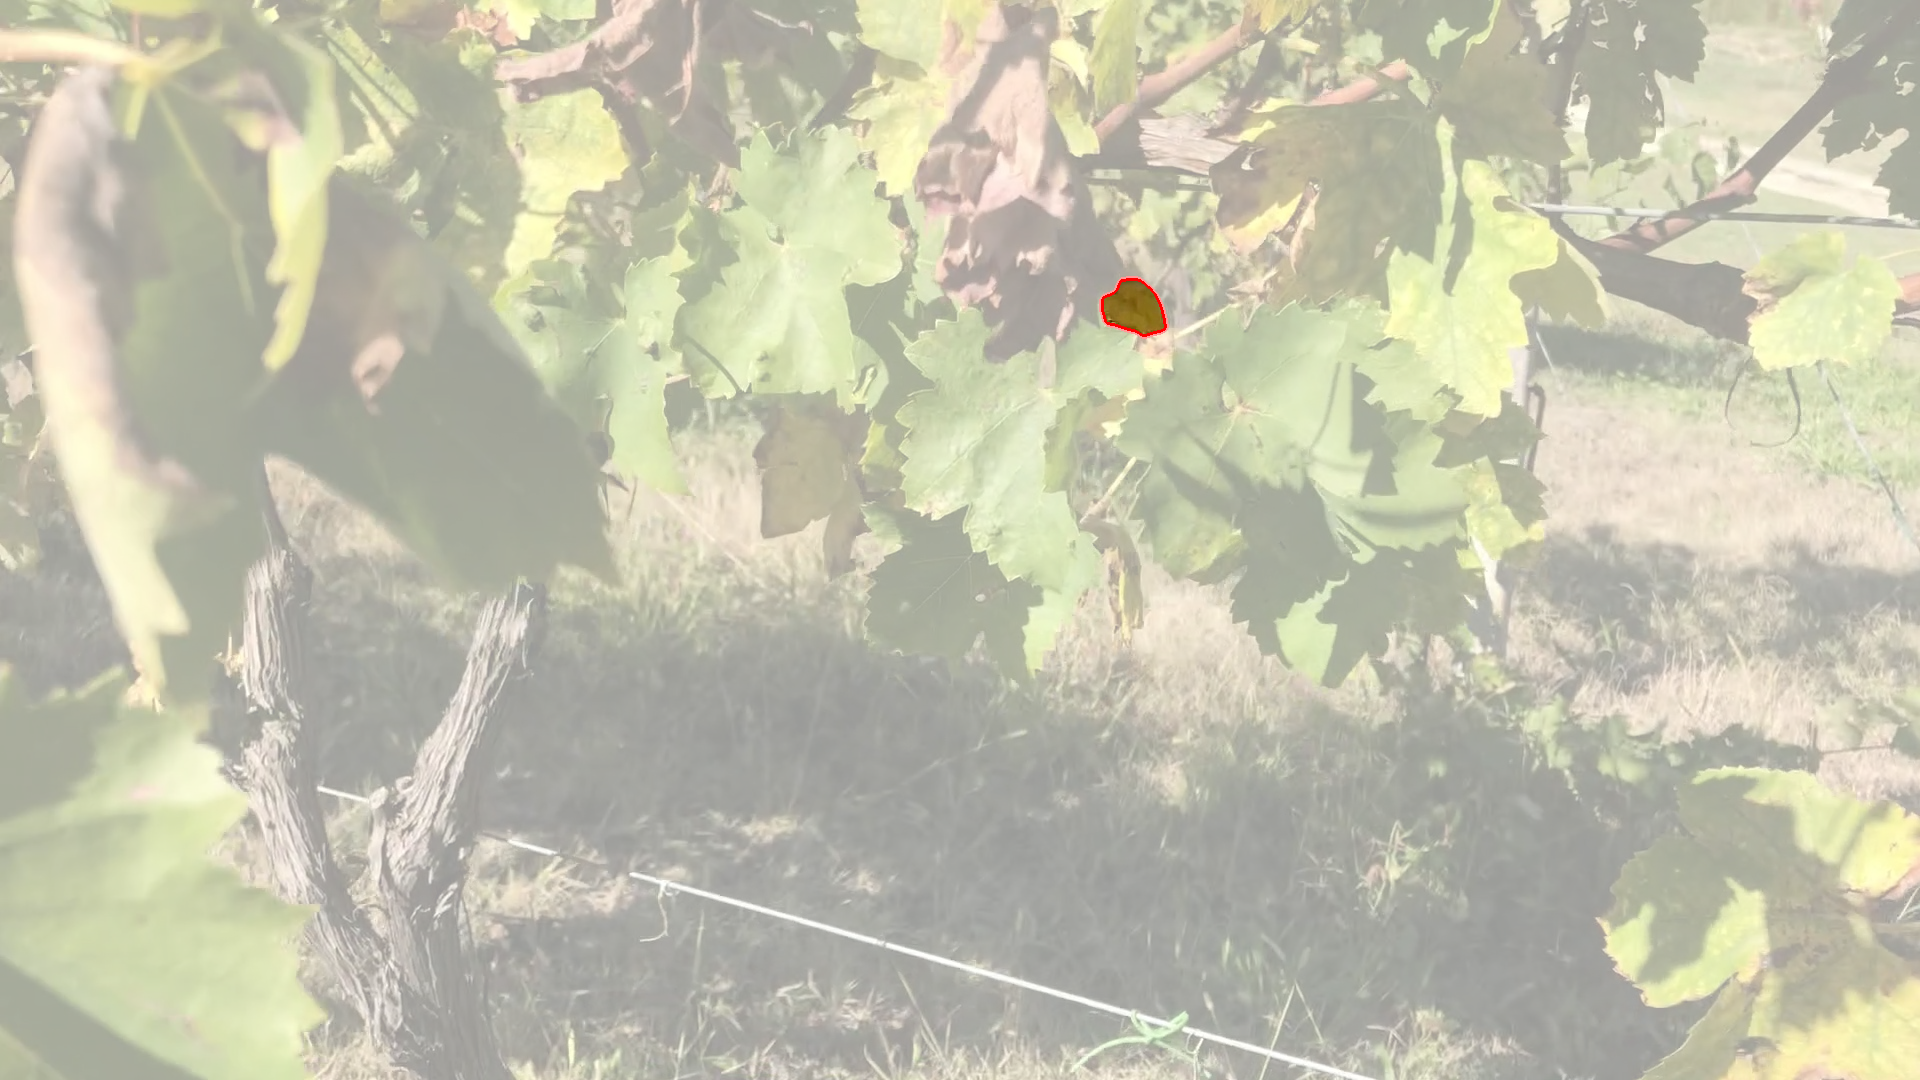
\includegraphics[width=\linewidth]{imgs/20_over_healthy_033_cam3.png}
%\caption{}
%\label{fig:sam1d}
%\end{subfigure}%%%%%%%%%%%%%%%%%%%%%%%%%%%%%

\begin{subfigure}[b]{.66\linewidth}
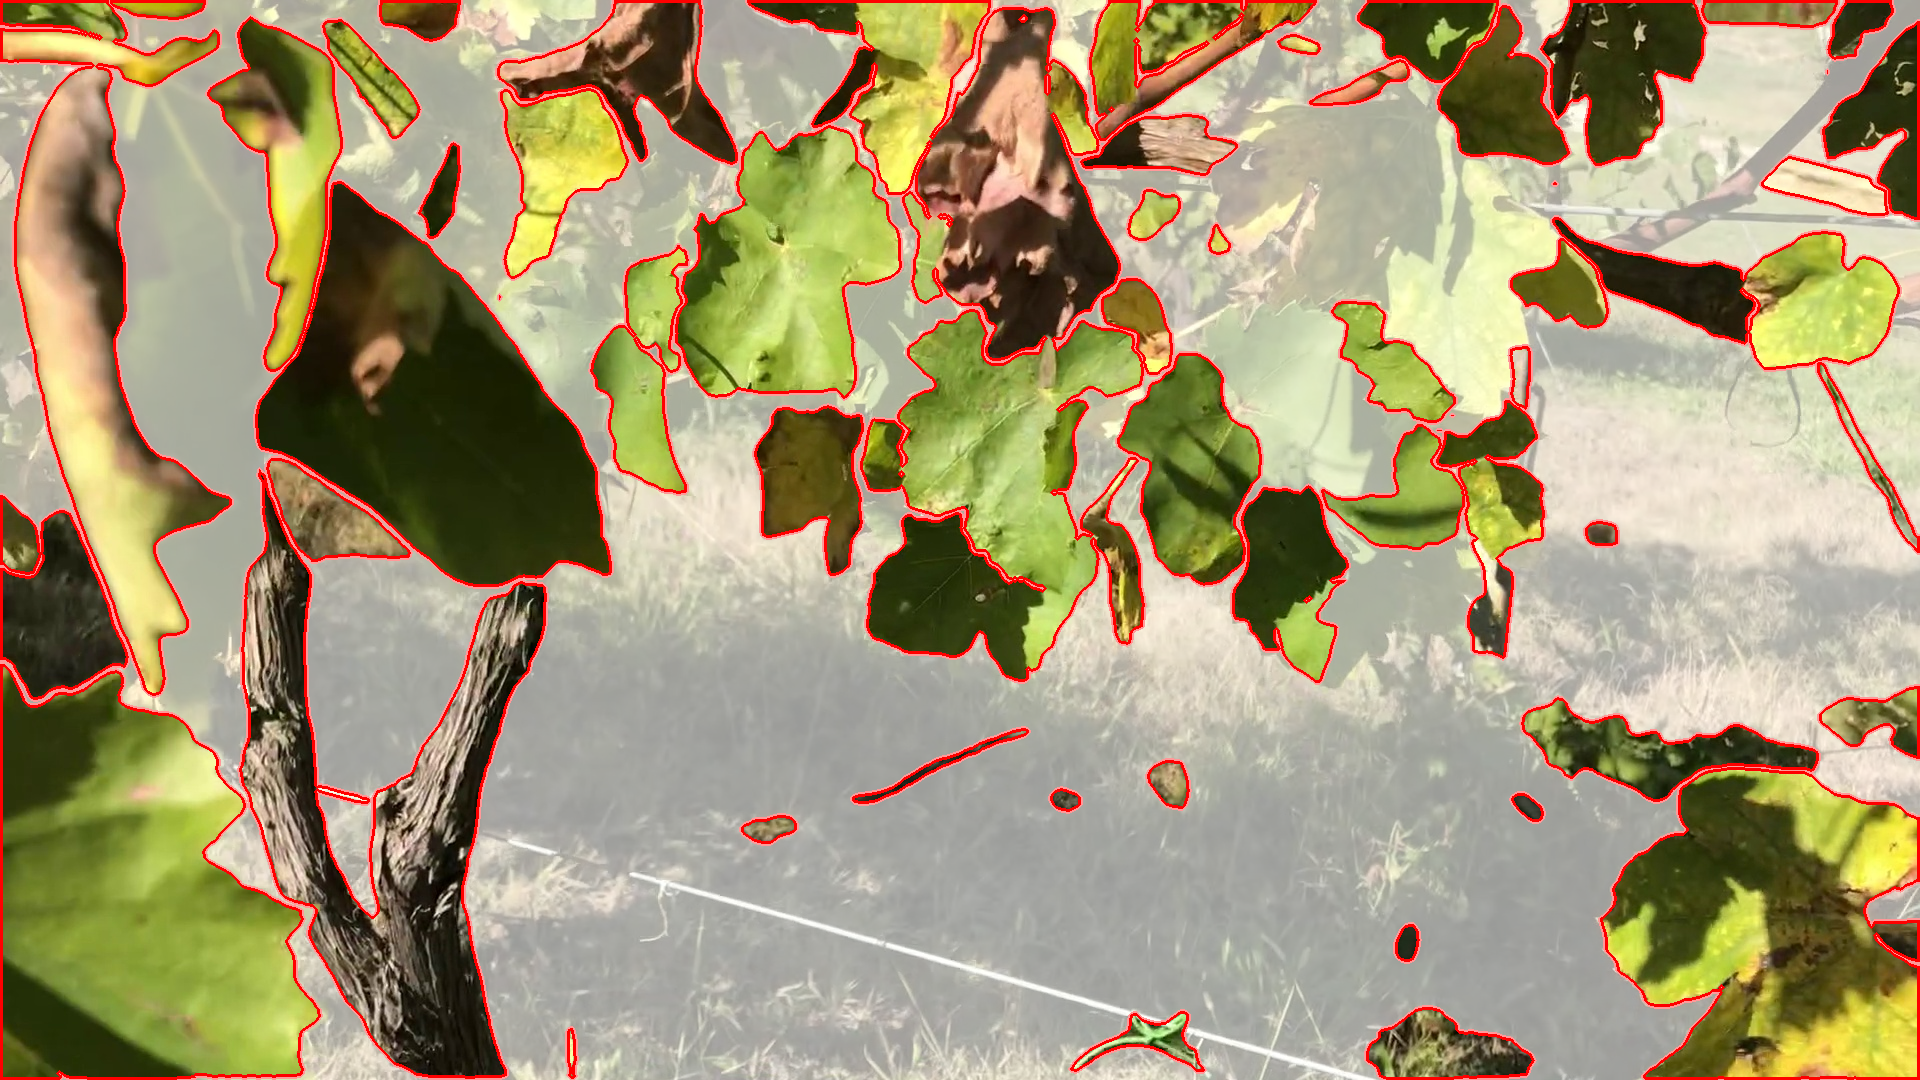
\includegraphics[width=\linewidth]{imgs/healthy_033_cam3_mask_over_healthy_033_cam3.png}
\caption{}
\label{fig:sam1e}
\end{subfigure}
\label{fig:individual_SAM_mask_and_their_union}
\caption{Two masks produced by SAM in automatic mode on {\color{red} healthy1.jpg} and the union of all masks produced for the same image.}
\end{figure}

\begin{table}[h!]
\centering
\begin{tabular}{|p{2.0cm}|p{1.0cm}|p{1.0cm}|p{1.0cm}|p{1.0cm}|p{1.0cm}|p{1.0cm}|p{1.0cm}|}
\hline
\makecell{\textbf{Image Name}} & \makecell{\textbf{IoU}} & \makecell{\textbf{DC}} & \makecell{\textbf{PA}} & \makecell{\textbf{Prec}} & \makecell{\textbf{Rec}} & \makecell{\textbf{F1}} \\
\hline
healthy1.jpg & ... & ... & ... & ... & ... & ... \\
\hline
healthy2.jpg & ... & ... & ... & ... & ... & ... \\
\hline
healthy3.jpg & ... & ... & ... & ... & ... & ... \\
\hline
healthy4.jpg & ... & ... & ... & ... & ... & ... \\
\hline
healthy5.jpg & ... & ... & ... & ... & ... & ... \\
\hline
esca1.jpg & ... & ... & ... & ... & ... & ... \\
\hline
esca2.jpg & ... & ... & ... & ... & ... & ... \\
\hline
esca3.jpg & ... & ... & ... & ... & ... & ... \\
\hline
esca4.jpg & ... & ... & ... & ... & ... & ... \\
\hline
esca5.jpg & ... & ... & ... & ... & ... & ... \\
\hline
\end{tabular}
\caption{Evaluation of semantic segmentation performet by SAM in automatic mode}
\label{tab:segmentation_evaluation_SAM_automatic}
\end{table}

\begin{table}[h!]
\centering
\begin{tabular}{|p{2.0cm}|p{1.0cm}|p{1.0cm}|p{1.0cm}|p{1.0cm}|p{1.0cm}|p{1.0cm}|p{1.0cm}|}
\hline
\makecell{\textbf{Image Name}} & \makecell{\textbf{IoU}} & \makecell{\textbf{DC}} & \makecell{\textbf{PA}} & \makecell{\textbf{Prec}} & \makecell{\textbf{Rec}} & \makecell{\textbf{F1}} \\
\hline
healthy1.jpg & ... & ... & ... & ... & ... & ... \\
\hline
healthy2.jpg & ... & ... & ... & ... & ... & ... \\
\hline
healthy3.jpg & ... & ... & ... & ... & ... & ... \\
\hline
healthy4.jpg & ... & ... & ... & ... & ... & ... \\
\hline
healthy5.jpg & ... & ... & ... & ... & ... & ... \\
\hline
esca1.jpg & ... & ... & ... & ... & ... & ... \\
\hline
esca2.jpg & ... & ... & ... & ... & ... & ... \\
\hline
esca3.jpg & ... & ... & ... & ... & ... & ... \\
\hline
esca4.jpg & ... & ... & ... & ... & ... & ... \\
\hline
esca5.jpg & ... & ... & ... & ... & ... & ... \\
\hline
\end{tabular}
\caption{Evaluation of semantic segmentation performed by SAM in bounding box mode}
\label{tab:segmentation_evaluation_SAM_bbox}
\end{table}

\begin{table}[h!]
\centering
\begin{tabular}{|p{2.0cm}|p{1.0cm}|p{1.0cm}|p{1.0cm}|p{1.0cm}|p{1.0cm}|p{1.0cm}|p{1.0cm}|}
\hline
\makecell{\textbf{Image Name}} & \makecell{\textbf{IoU}} & \makecell{\textbf{DC}} & \makecell{\textbf{PA}} & \makecell{\textbf{Prec}} & \makecell{\textbf{Rec}} & \makecell{\textbf{F1}} \\
\hline
healthy1.jpg & ... & ... & ... & ... & ... & ... \\
\hline
healthy2.jpg & ... & ... & ... & ... & ... & ... \\
\hline
healthy3.jpg & ... & ... & ... & ... & ... & ... \\
\hline
healthy4.jpg & ... & ... & ... & ... & ... & ... \\
\hline
healthy5.jpg & ... & ... & ... & ... & ... & ... \\
\hline
esca1.jpg & ... & ... & ... & ... & ... & ... \\
\hline
esca2.jpg & ... & ... & ... & ... & ... & ... \\
\hline
esca3.jpg & ... & ... & ... & ... & ... & ... \\
\hline
esca4.jpg & ... & ... & ... & ... & ... & ... \\
\hline
esca5.jpg & ... & ... & ... & ... & ... & ... \\
\hline
\end{tabular}
\caption{Evaluation of semantic segmentation performed by SAM in point mode}
\label{tab:segmentation_evaluation_SAM_point}
\end{table}

\subsection{Segmentation of vine images with U-Net}

In order to test semantic segmentation of vine images with U-Net we used the APEER ML toolkit by {\color{red}{Zeiss\textsuperscript{\tiny\textregistered}} ?}. The toolkit offers the possibility to train a U-Net with EfficientNet encoder that was then used to perform semantic segmentation on all 1770 images of the ESCA dataset. All generated masks were then downloaded.

\begin{figure}[h!]
\centering
\begin{subfigure}[b]{.47\linewidth}

\includegraphics[width=\linewidth]{imgs/placeholder.jpg}
\caption{}
\end{subfigure}
\begin{subfigure}[b]{.47\linewidth}
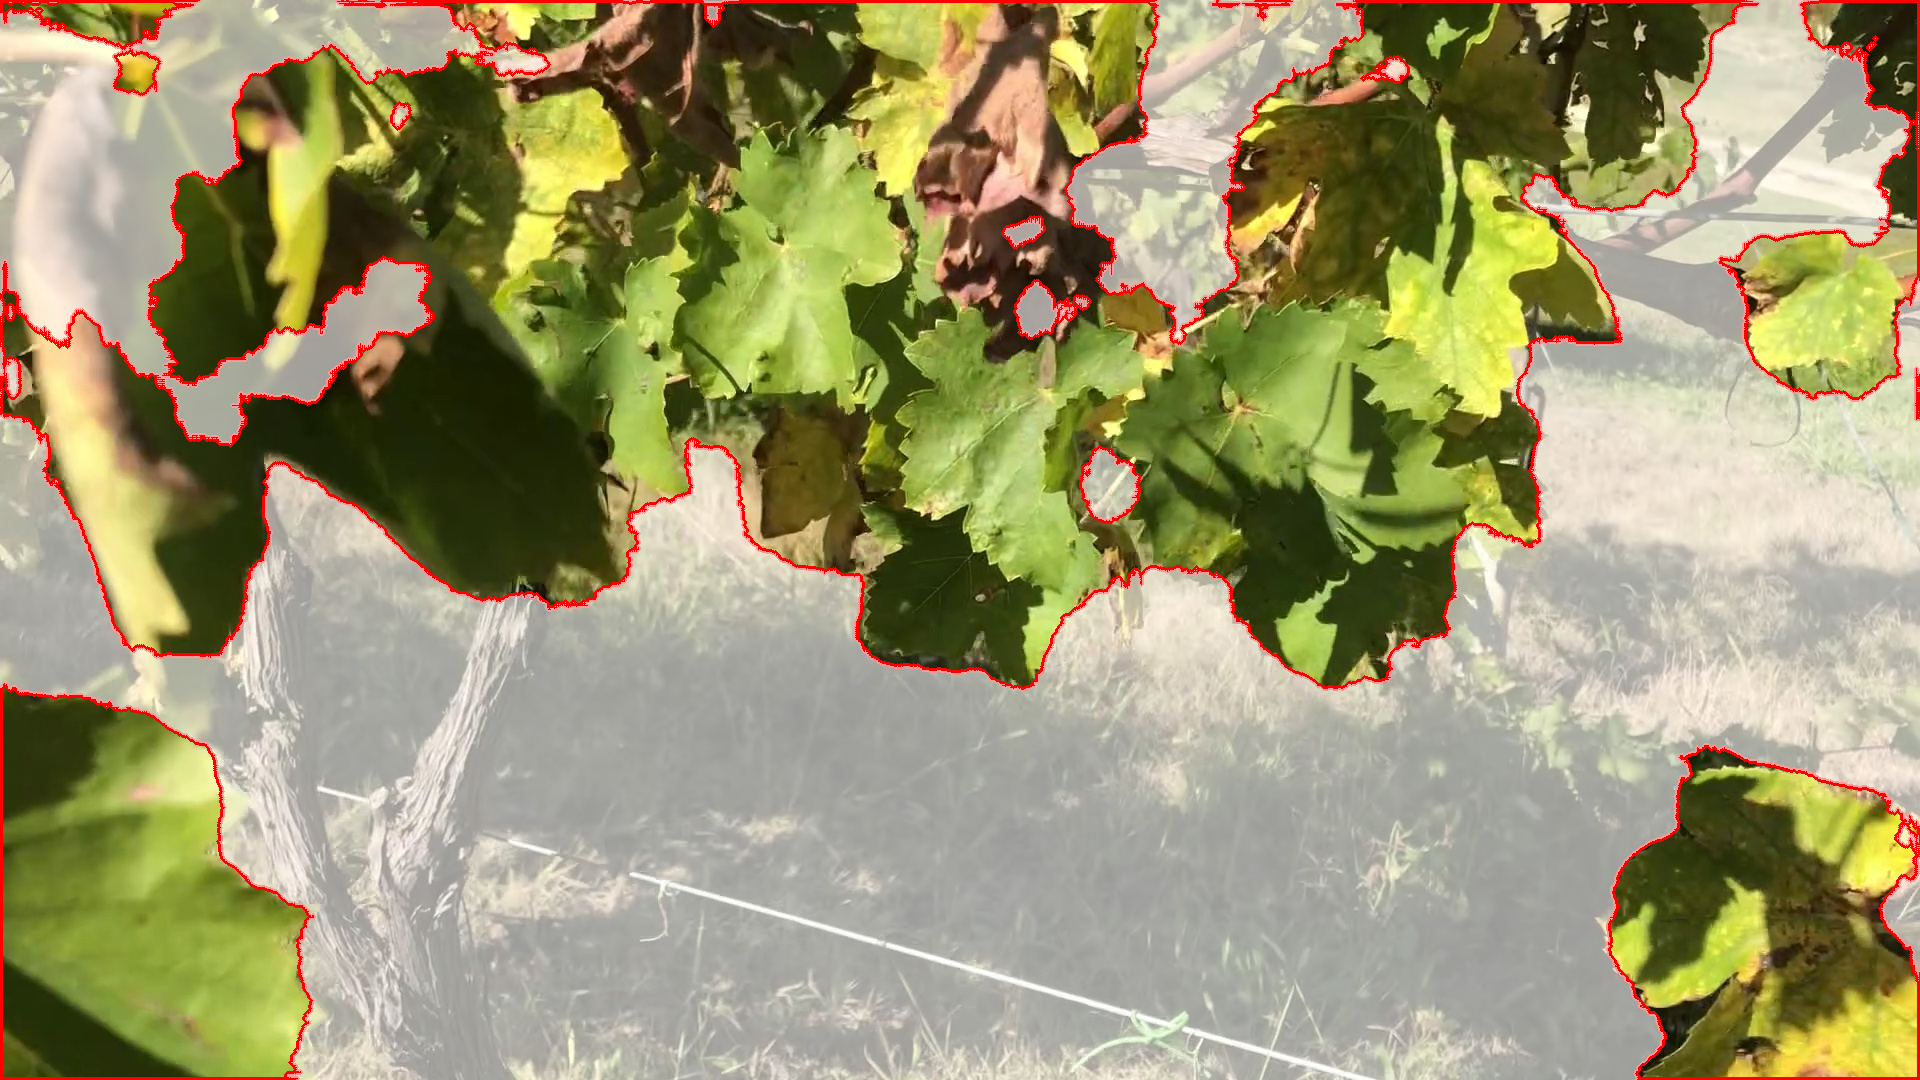
\includegraphics[width=\linewidth]{imgs/healthy_033_cam3_finalprediction_over_healthy_033_cam3.png}
\caption{}
\end{subfigure}
\caption{Segmentation produced by U-Net on {\color{red}healthy.jpg} and {\color{red}esca1.jpg}}
\label{fig:unet_segmentation}
\end{figure}

\begin{table}[h!]
\centering
\begin{tabular}{|p{3.0cm}|p{3.0cm}|p{3.7cm}|}
\hline
\makecell{\textbf{Image folder}}
&
\makecell{\textbf{Number of images}}
&
\makecell{\textbf{Image segmentation time}} \\
\hline
Esca     & 888 & ???  \\
\hline
Healthy & 882 &  ???  \\
\hline
\end{tabular}
\caption{Image segmentation time with UNet}
\label{tab:image_segmentation_on_UNet_automatic}
\end{table}

\begin{table}[h!]
\centering
\begin{tabular}{|p{2.0cm}|p{1.0cm}|p{1.0cm}|p{1.0cm}|p{1.0cm}|p{1.0cm}|p{1.0cm}|p{1.0cm}|}
\hline
\makecell{\textbf{Image Name}} & \makecell{\textbf{IoU}} & \makecell{\textbf{DC}} & \makecell{\textbf{PA}} & \makecell{\textbf{Prec}} & \makecell{\textbf{Rec}} & \makecell{\textbf{F1}} \\
\hline
image1.jpg & ... & ... & ... & ... & ... & ... \\
\hline
image2.jpg & ... & ... & ... & ... & ... & ... \\
\hline
image3.jpg & ... & ... & ... & ... & ... & ... \\
\hline
image4.jpg & ... & ... & ... & ... & ... & ... \\
\hline
image5.jpg & ... & ... & ... & ... & ... & ... \\
\hline
image6.jpg & ... & ... & ... & ... & ... & ... \\
\hline
image7.jpg & ... & ... & ... & ... & ... & ... \\
\hline
image8.jpg & ... & ... & ... & ... & ... & ... \\
\hline
image9.jpg & ... & ... & ... & ... & ... & ... \\
\hline
image10.jpg & ... & ... & ... & ... & ... & ... \\
\hline
\end{tabular}
\caption{Evaluation of semantic segmentation performed by UNet.}
\label{tab:segmentation_evaluation_UNet}
\end{table}

% \subsection{Future work}
% 

% multi-mask output could be useful in some nested segmentation tasks, brain tumor
\section{Discussion and Conclusion}

{\color{red} 
Lorem ipsum dolor sit amet, consectetur adipiscing elit, sed do eiusmod tempor incididunt ut labore et dolore magna aliqua. Ut enim ad minim veniam, quis nostrud exercitation ullamco laboris nisi ut aliquip ex ea commodo consequat. Duis aute irure dolor in reprehenderit in voluptate velit esse cillum dolore eu fugiat nulla pariatur. Excepteur sint occaecat cupidatat non proident, sunt in culpa qui officia deserunt mollit anim id est laborum.

Lorem ipsum dolor sit amet, consectetur adipiscing elit, sed do eiusmod tempor incididunt ut labore et dolore magna aliqua. Ut enim ad minim veniam, quis nostrud exercitation ullamco laboris nisi ut aliquip ex ea commodo consequat. Duis aute irure dolor in reprehenderit in voluptate velit esse cillum dolore eu fugiat nulla pariatur. Excepteur sint occaecat cupidatat non proident, sunt in culpa qui officia deserunt mollit anim id est laborum.

Lorem ipsum dolor sit amet, consectetur adipiscing elit, sed do eiusmod tempor incididunt ut labore et dolore magna aliqua. Ut enim ad minim veniam, quis nostrud exercitation ullamco laboris nisi ut aliquip ex ea commodo consequat. Duis aute irure dolor in reprehenderit in voluptate velit esse cillum dolore eu fugiat nulla pariatur. Excepteur sint occaecat cupidatat non proident, sunt in culpa qui officia deserunt mollit anim id est laborum.
}




\subsubsection{Acknowledgements} 
The authors of this paper highly appreciate all the challenge organizers and owners for providing the public dataset to the community. We also thank Meta AI for making the source code of segment anything publicly available to the community. 

% ---- Bibliography ----
%
% BibTeX users should specify bibliography style 'splncs04'.
% References will then be sorted and formatted in the correct style.
\newpage
\bibliographystyle{splncs04}
\bibliography{ref}

\end{document}
